
\documentclass[11pt,letterpaper]{article}
\input{headings}
\newcommand \recipeName {Daniel's Tortilla Pasta}
\newcommand \fileName {TortillaPasta}
\chead{\recipeName}

\begin{document}
\input{title}

I developed this recipe as a quick meal for Daniel. Over time it became a staple in our house. The seasoning of the tortilla with olive oil, parmesan cheese, and black pepper makes it taste like pasta. Once you have \href{DanielsMeatSauce.html}{Daniel's meat sauce} in the freezer --- see separate recipe --- this is a meal that you can prepare in minutes.

\vspace{0.3in}
\begin{description}

\item[Ingredients:]\ \\
	\begin{itemize}
	\item 150 grams of \href{DanielsMeatSauce.html}{Daniel's meat sauce}
	\item 2 flour tortillas
	\item 1 Tablespoon of extra-virgin olive oil
	\item 2 Tablespoon of freshly grated parmesan cheese
	\item Freshly ground pepper
	\end{itemize}

\item[Procedure:]\ \\
	\begin{itemize}
	\item Heat up the meat sauce in the microwave oven until it is heated all the way through and steam is escaping from the dish.
	\item Cut up the tortilla into fine strips as shown in the pictures below. 
	\item Loosen up, with your fingers, any strips that stuck together during cutting into a mixing bowl. 
	\item  Sprinkle with the olive oil and mix well.
	\item Sprinkle the freshly grated parmesan cheese and the freshly ground pepper and stir gently.
	\item Verify that the meat sauce is still steaming, if not put back into the microwave for another minute.
	\item Assemble the dish into two warmed up soup bowls laying down a small layer of the "pasta" and then a small about of the sauce, repeating it three times in each bowl. 
	\item Put each bowl in the microwave for 30 seconds in full power and serve immediately. These 30 seconds will barely warm the tortilla strips without making them tough.
		\end{itemize}
\end{description}

\begin{table}
\begin{tabular}{cccc}
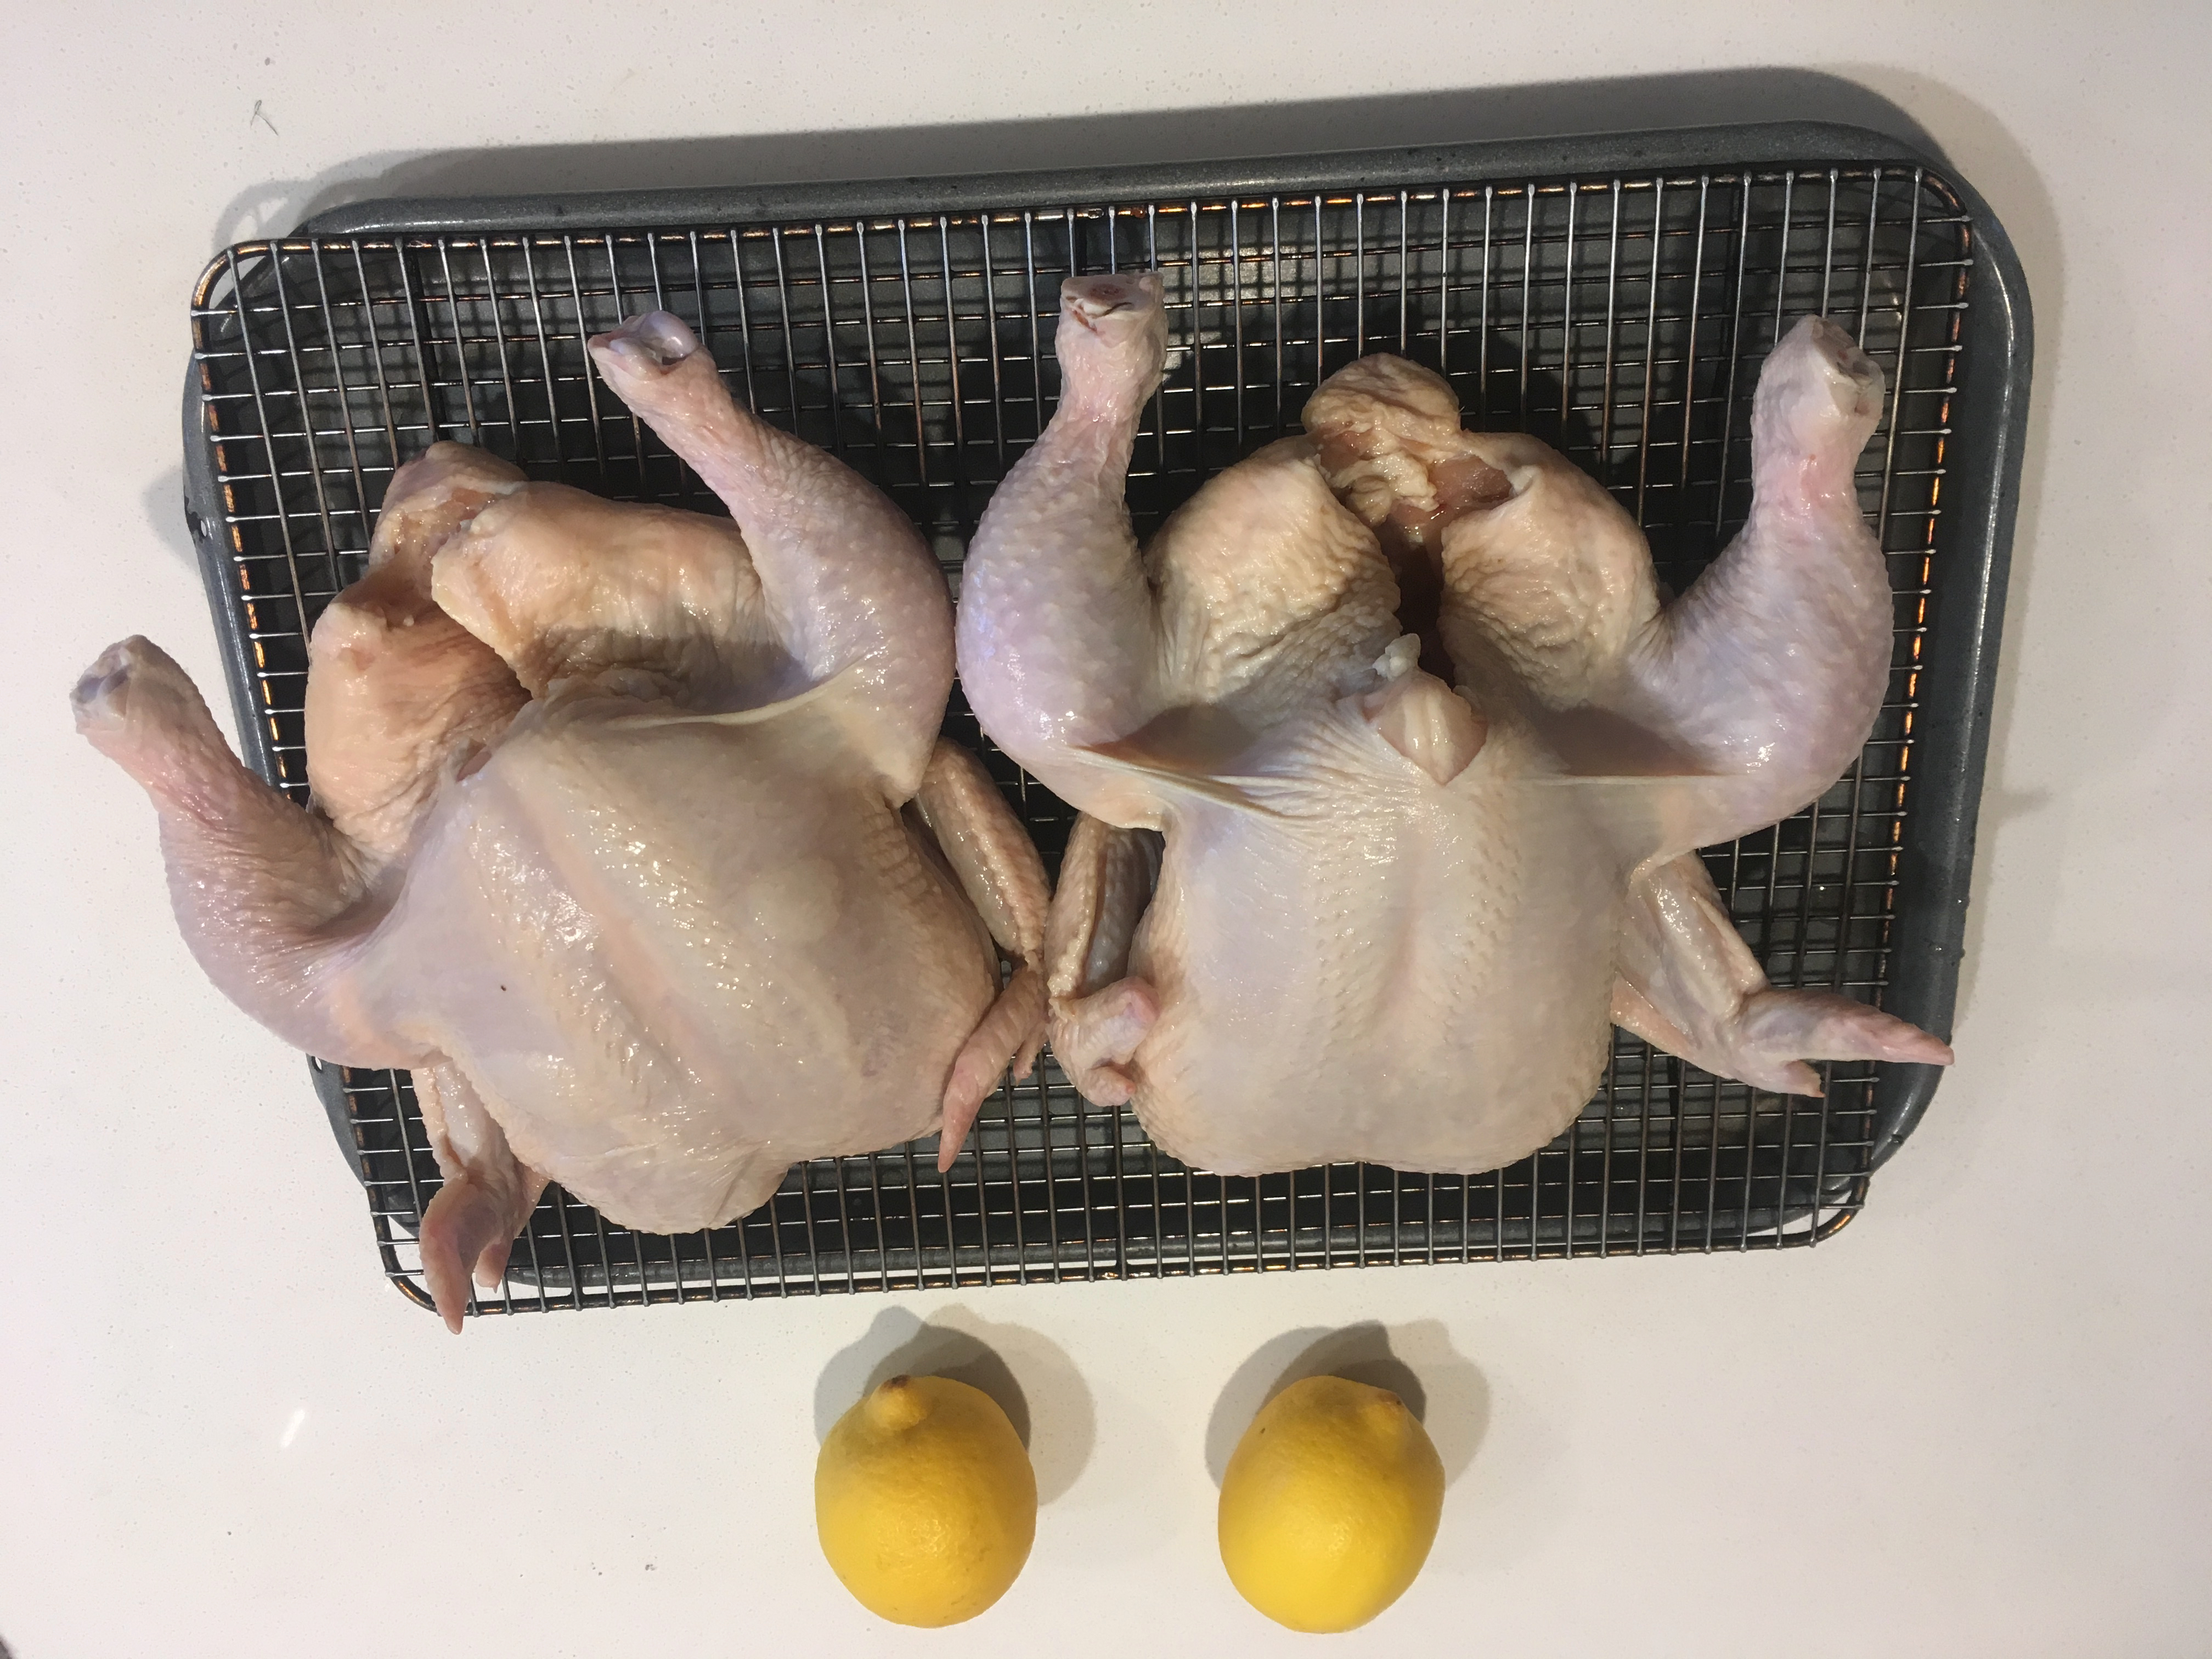
\includegraphics[width=0.25\textwidth]{\imageDir/\fileName/IMG_3197.jpg} &
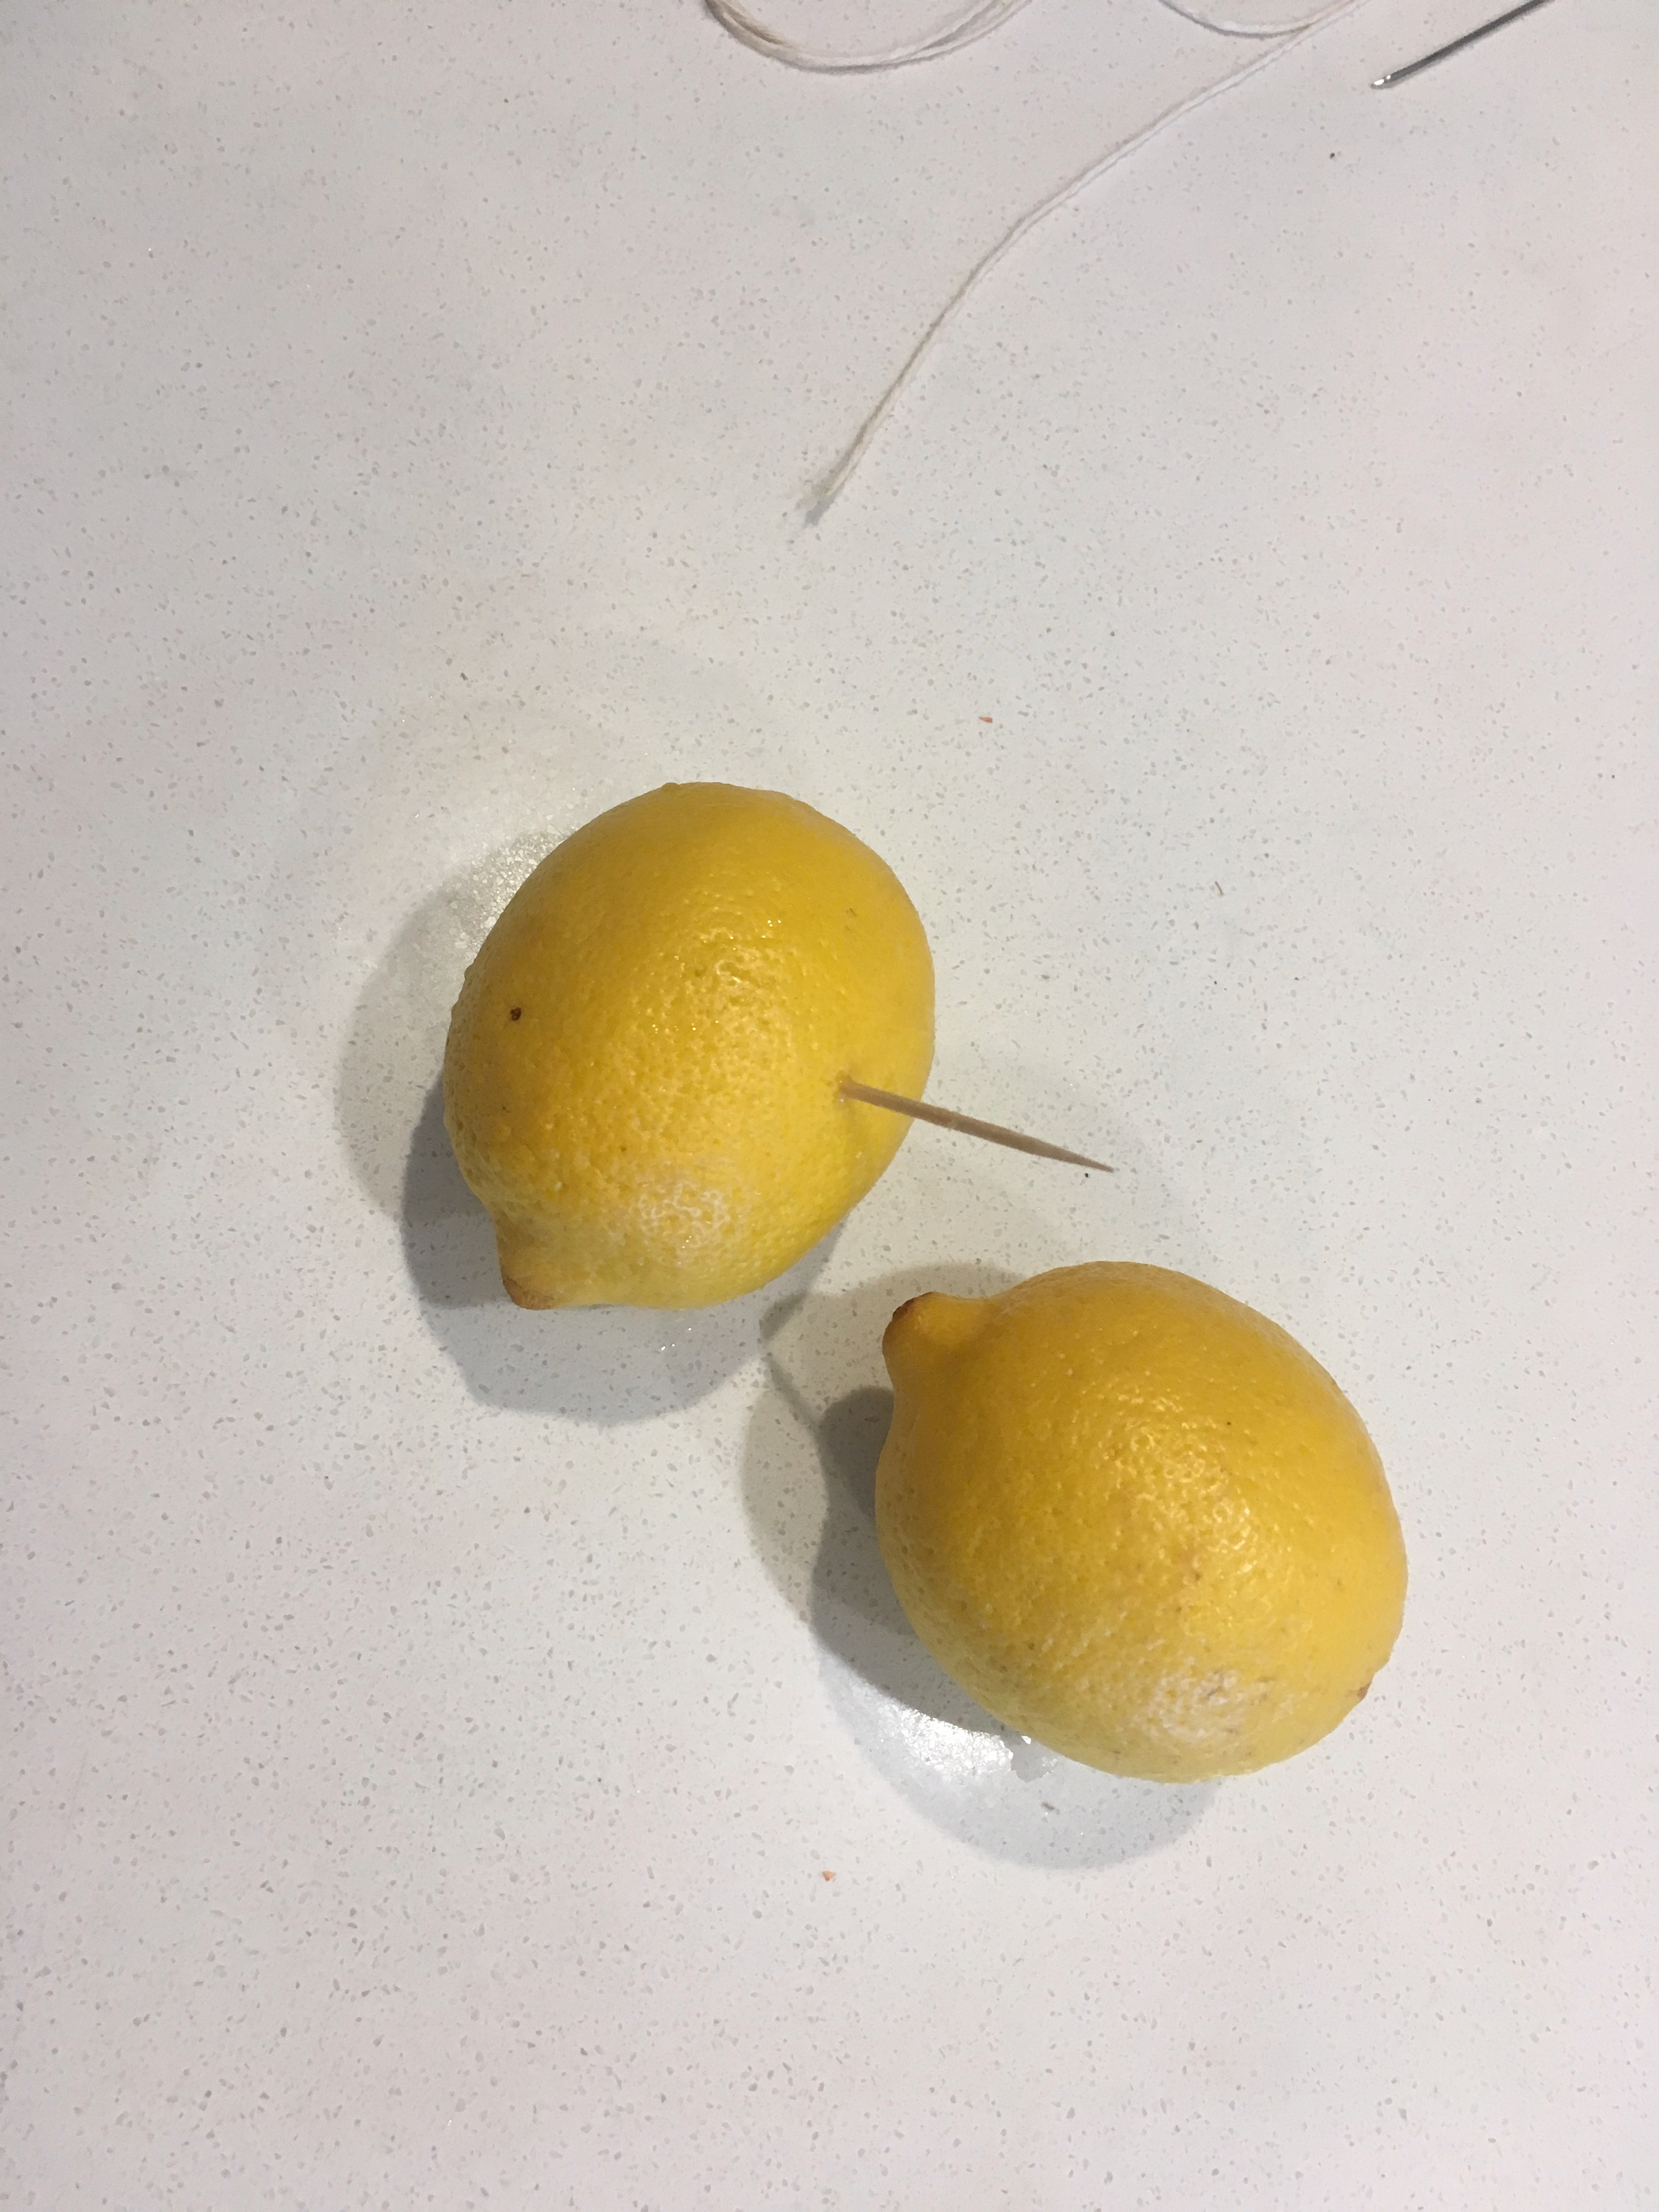
\includegraphics[width=0.25\textwidth]{\imageDir/\fileName/IMG_3212.jpg} &
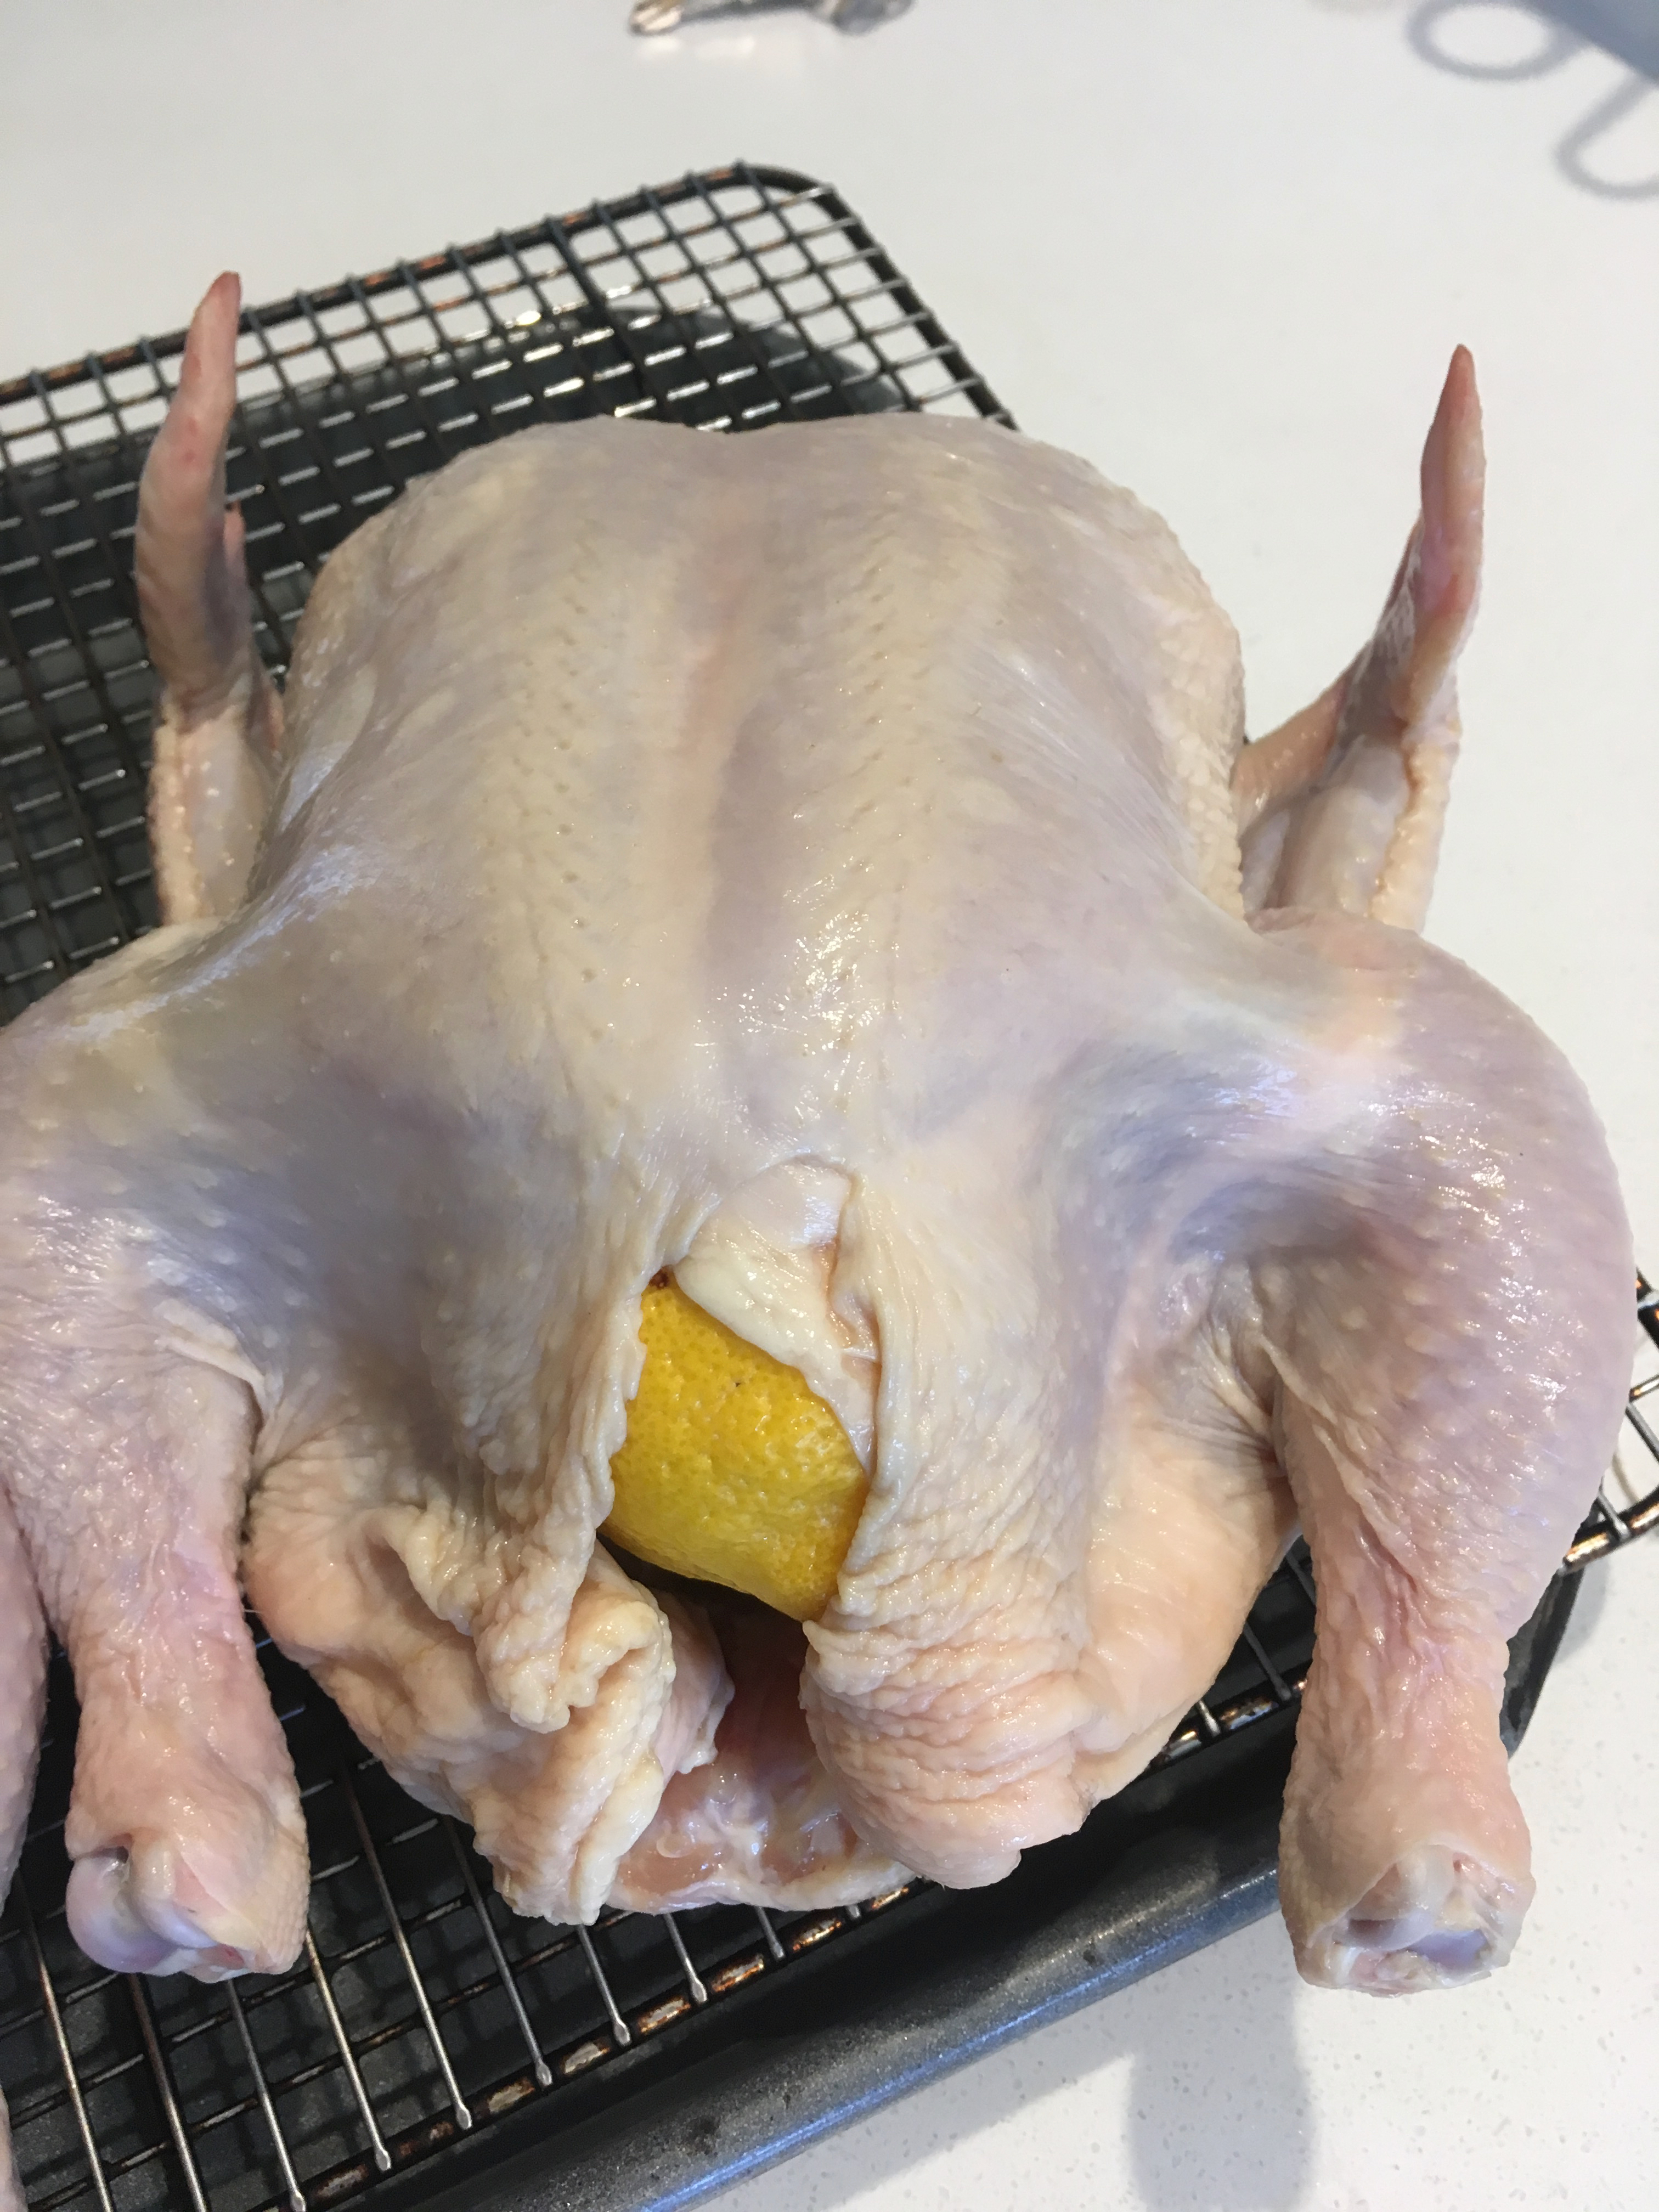
\includegraphics[width=0.25\textwidth]{\imageDir/\fileName/IMG_3213.jpg} \\
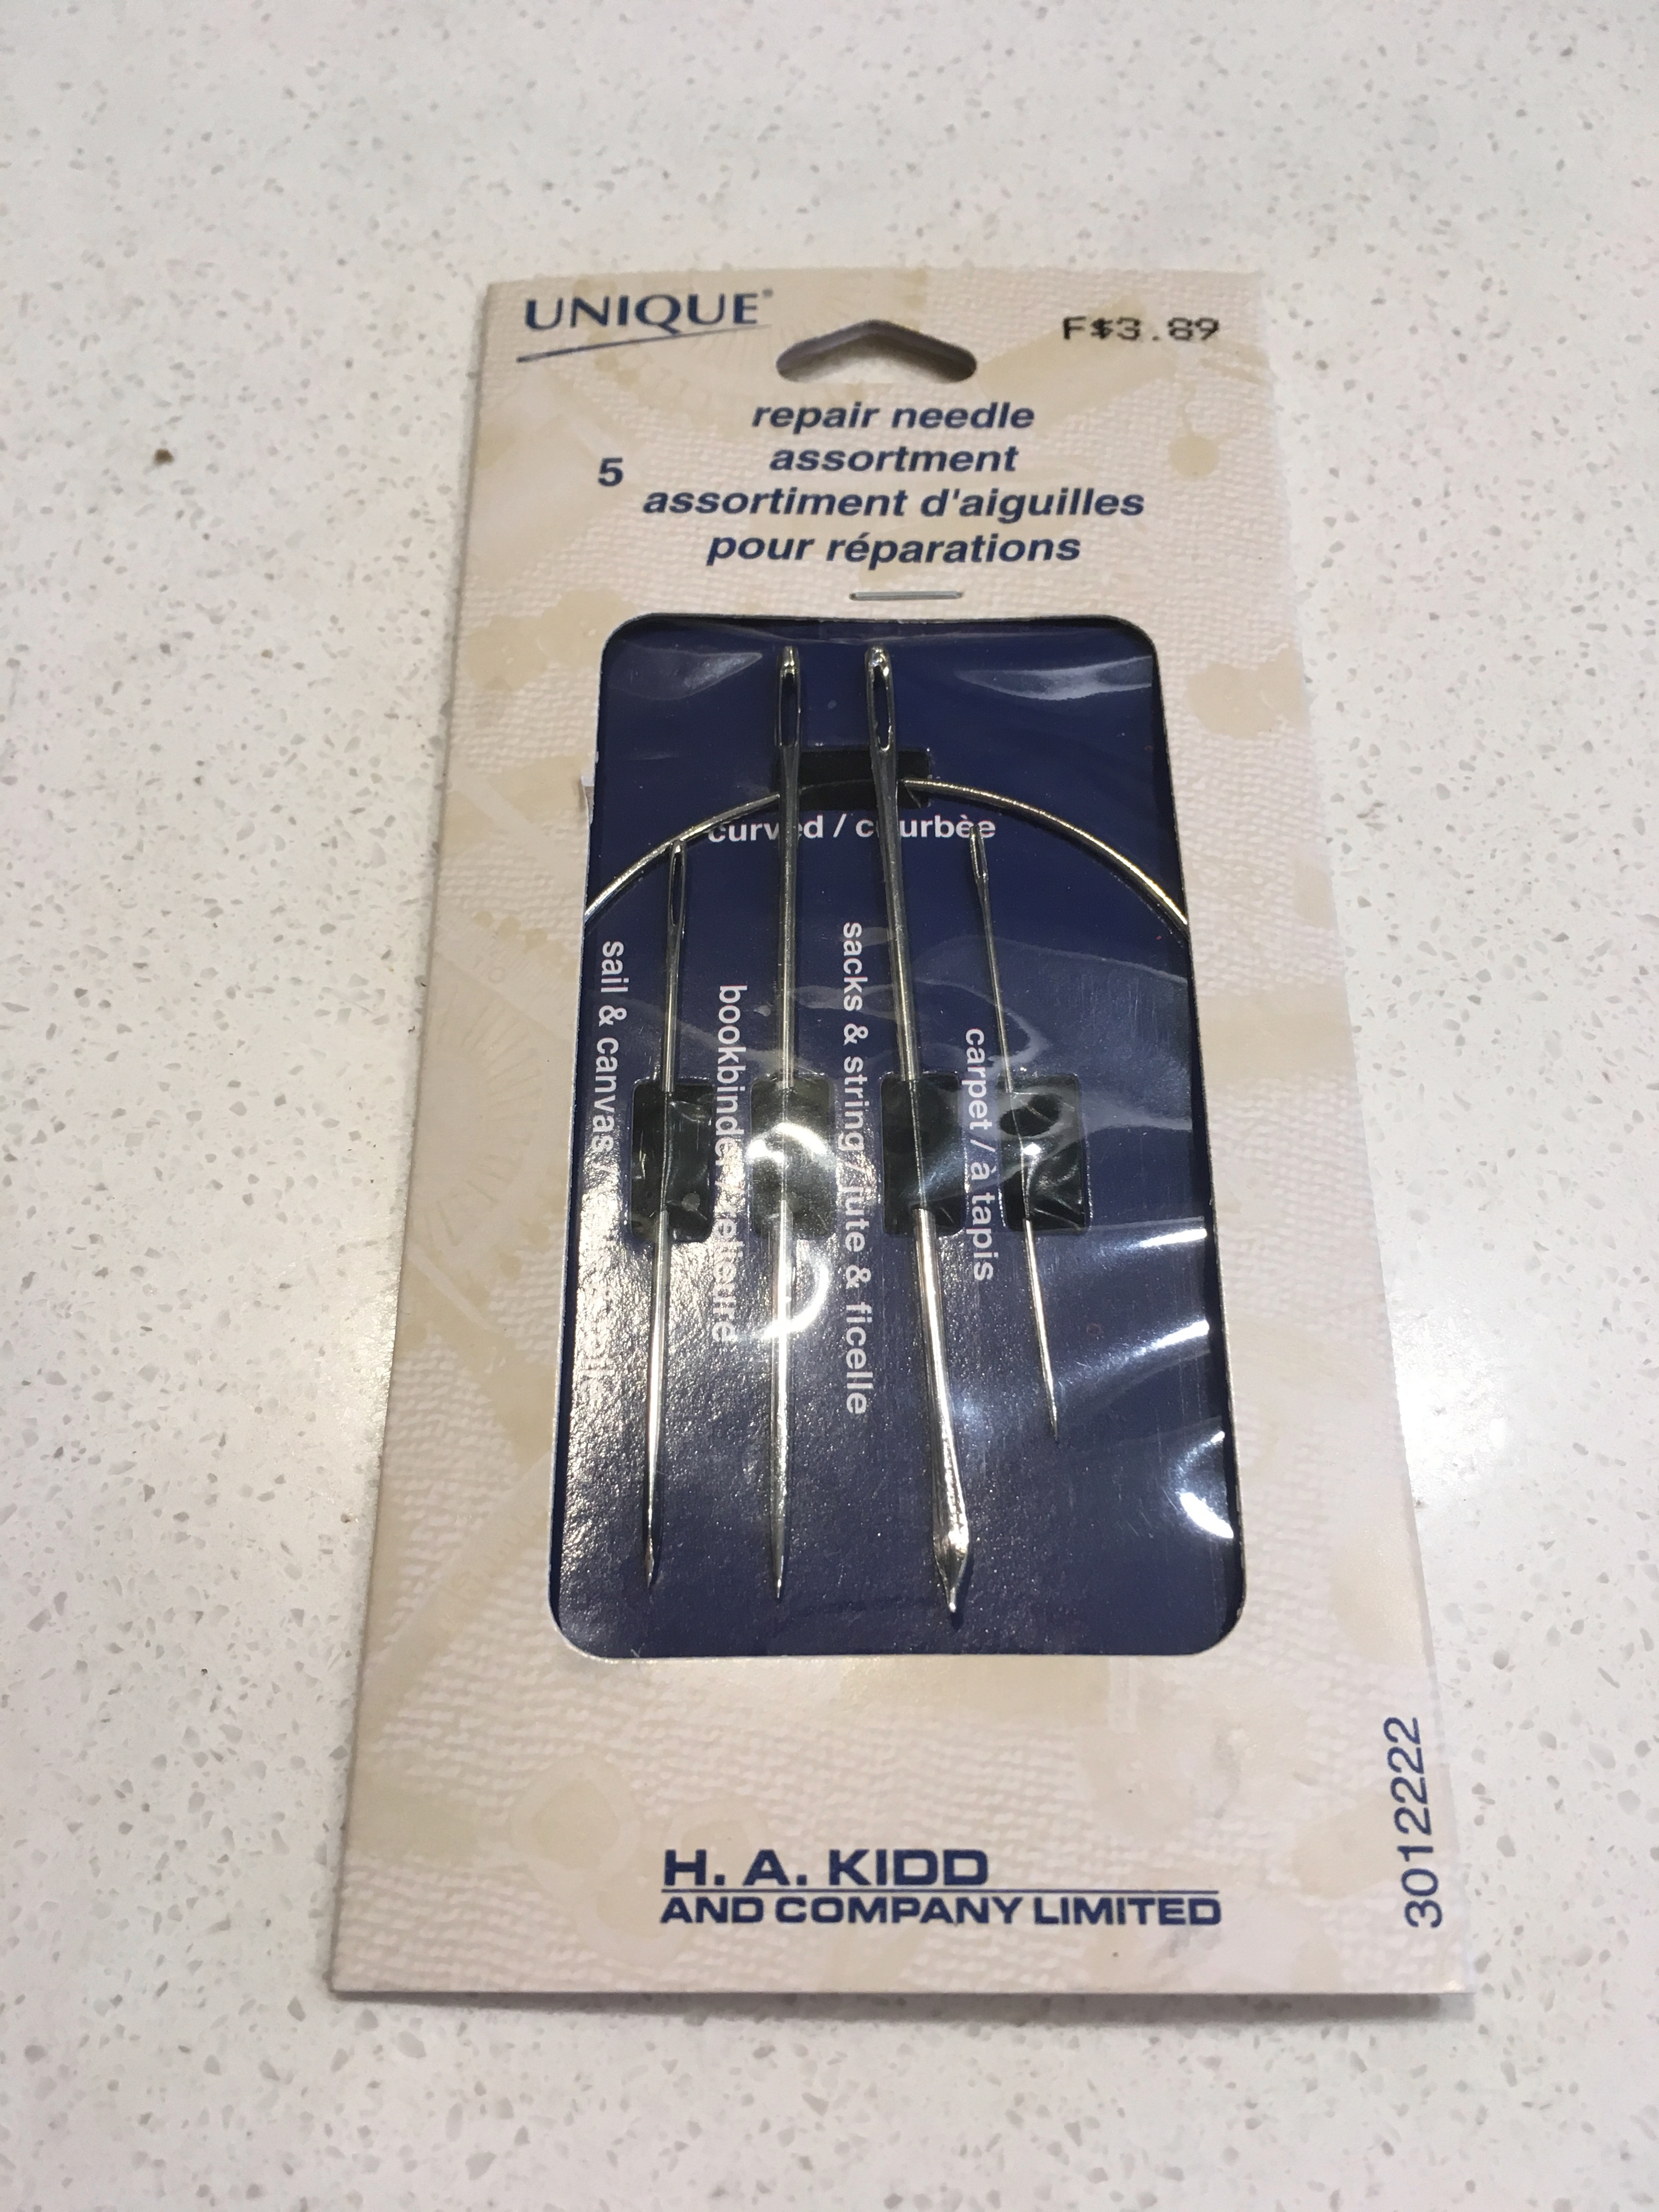
\includegraphics[width=0.25\textwidth]{\imageDir/\fileName/IMG_3206.jpg} &
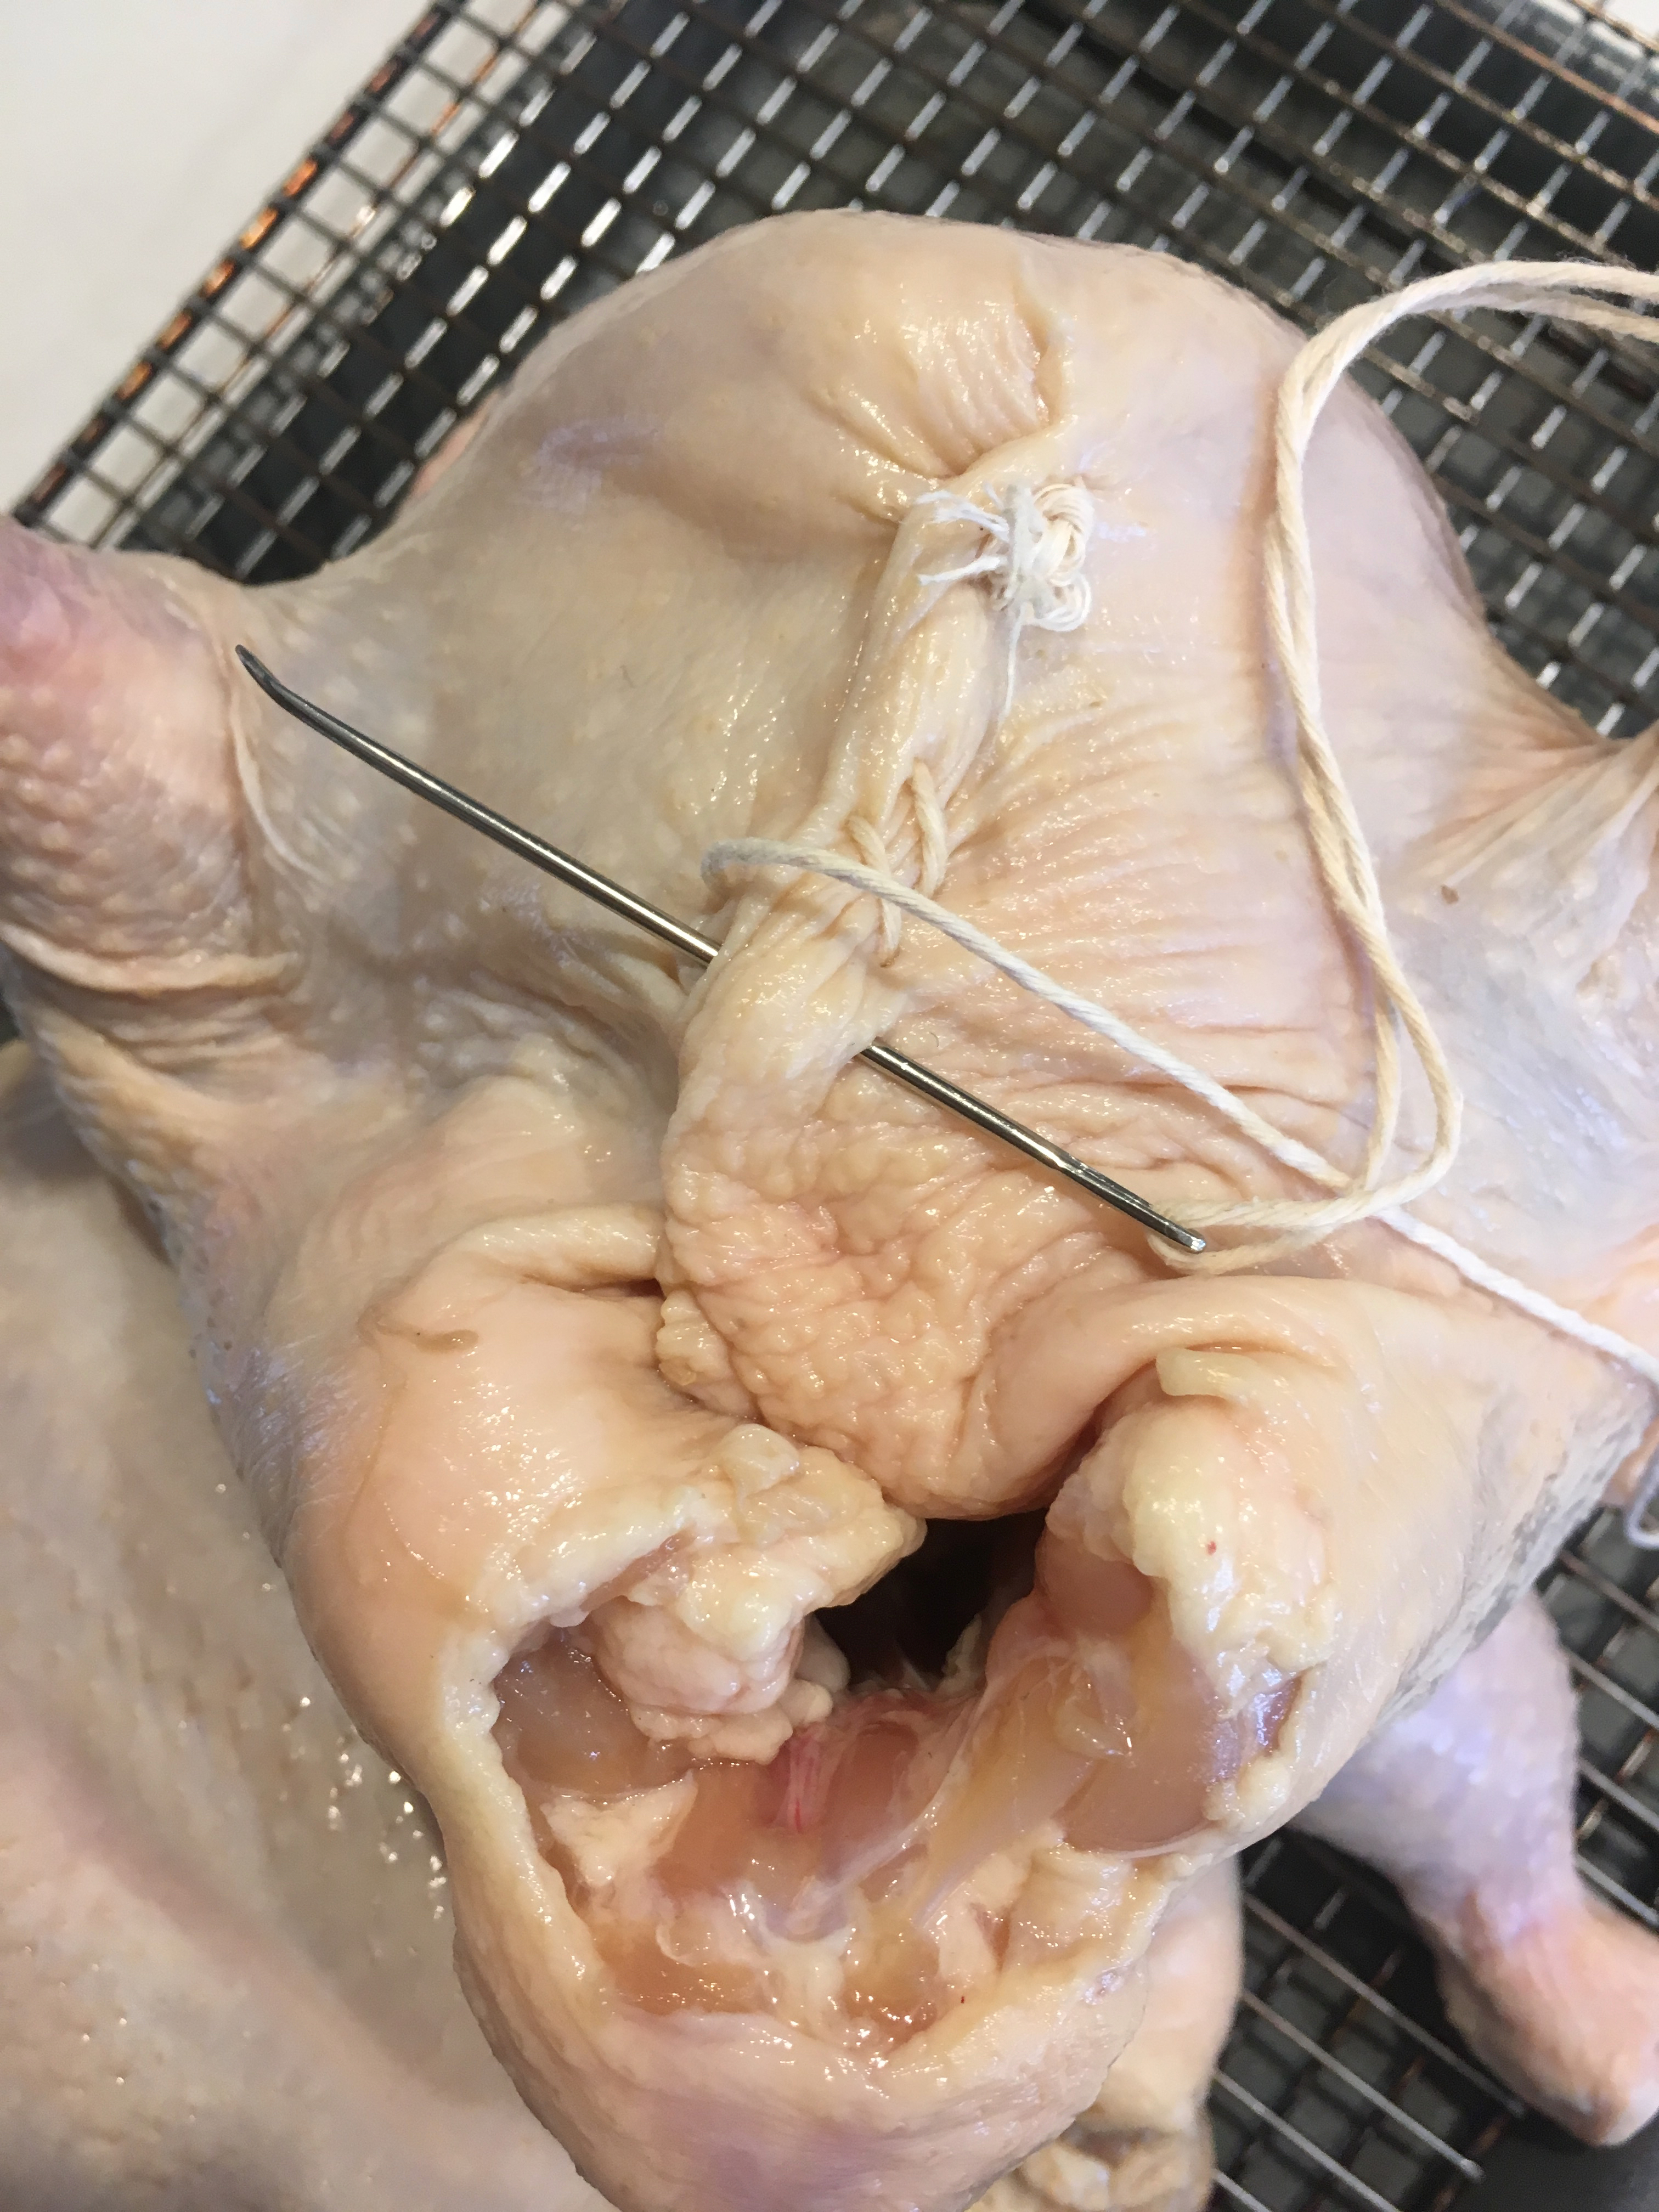
\includegraphics[width=0.25\textwidth]{\imageDir/\fileName/IMG_3214.jpg} &
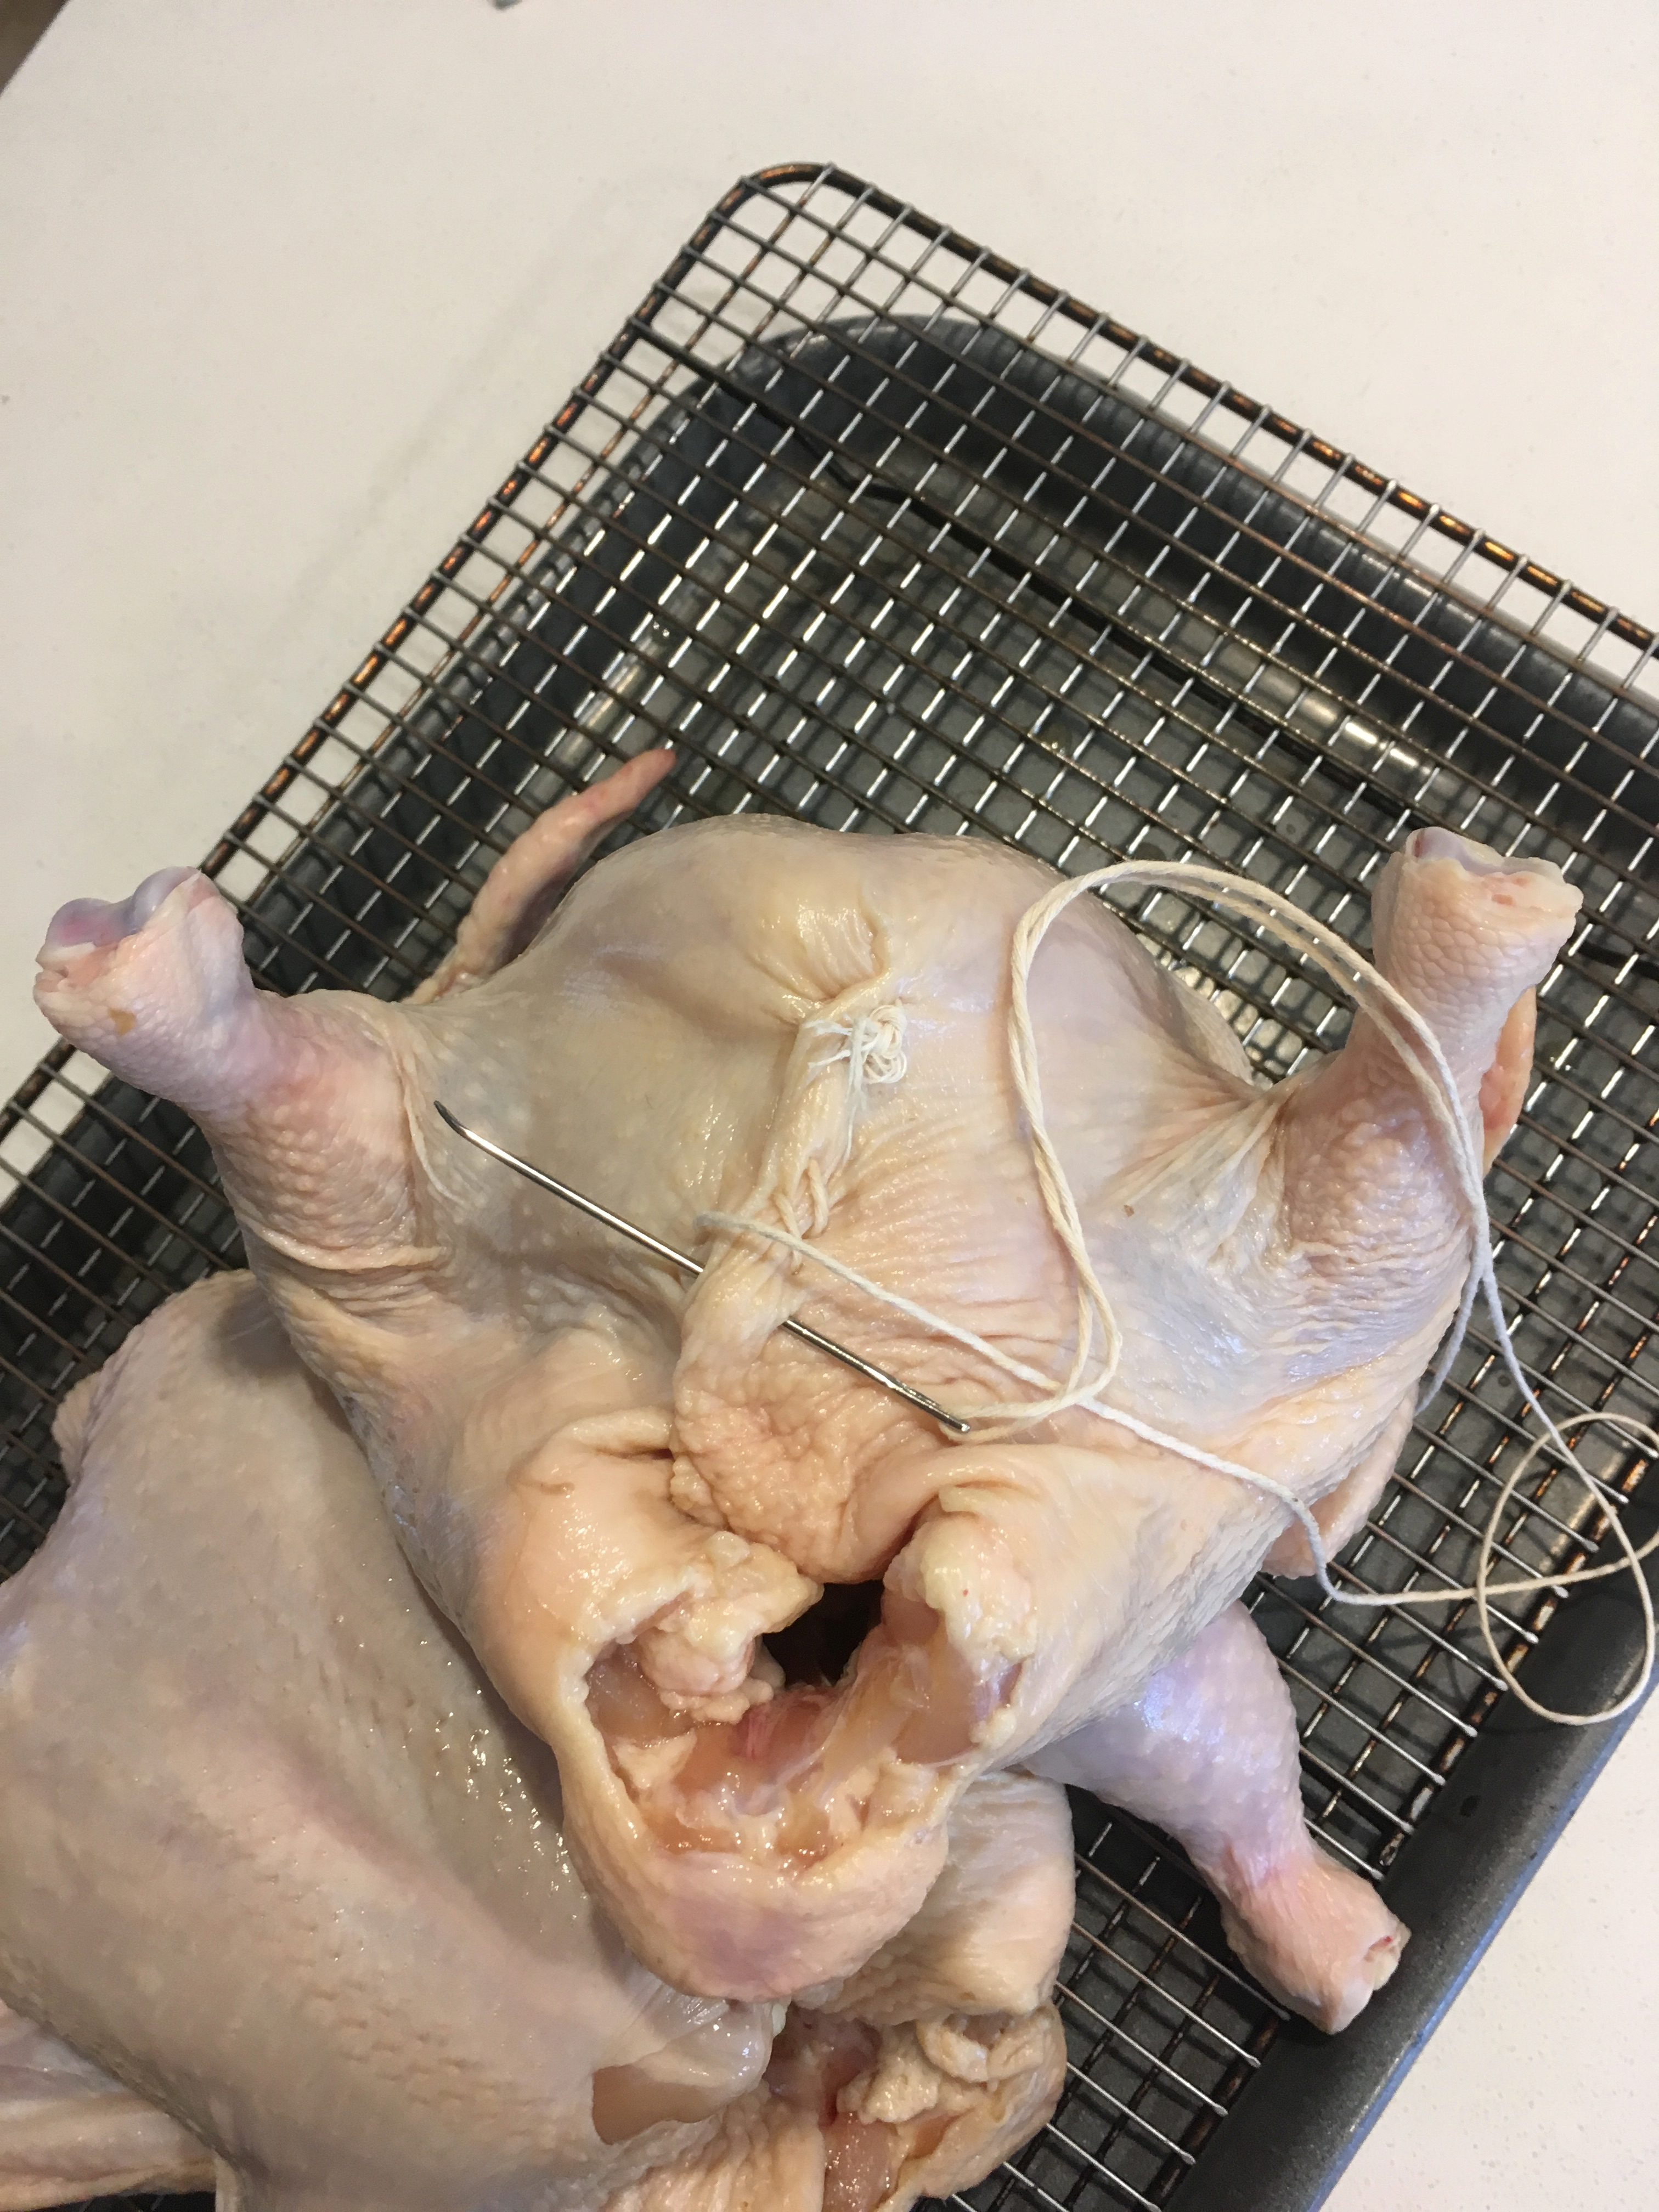
\includegraphics[width=0.25\textwidth]{\imageDir/\fileName/IMG_3216.jpg} \\
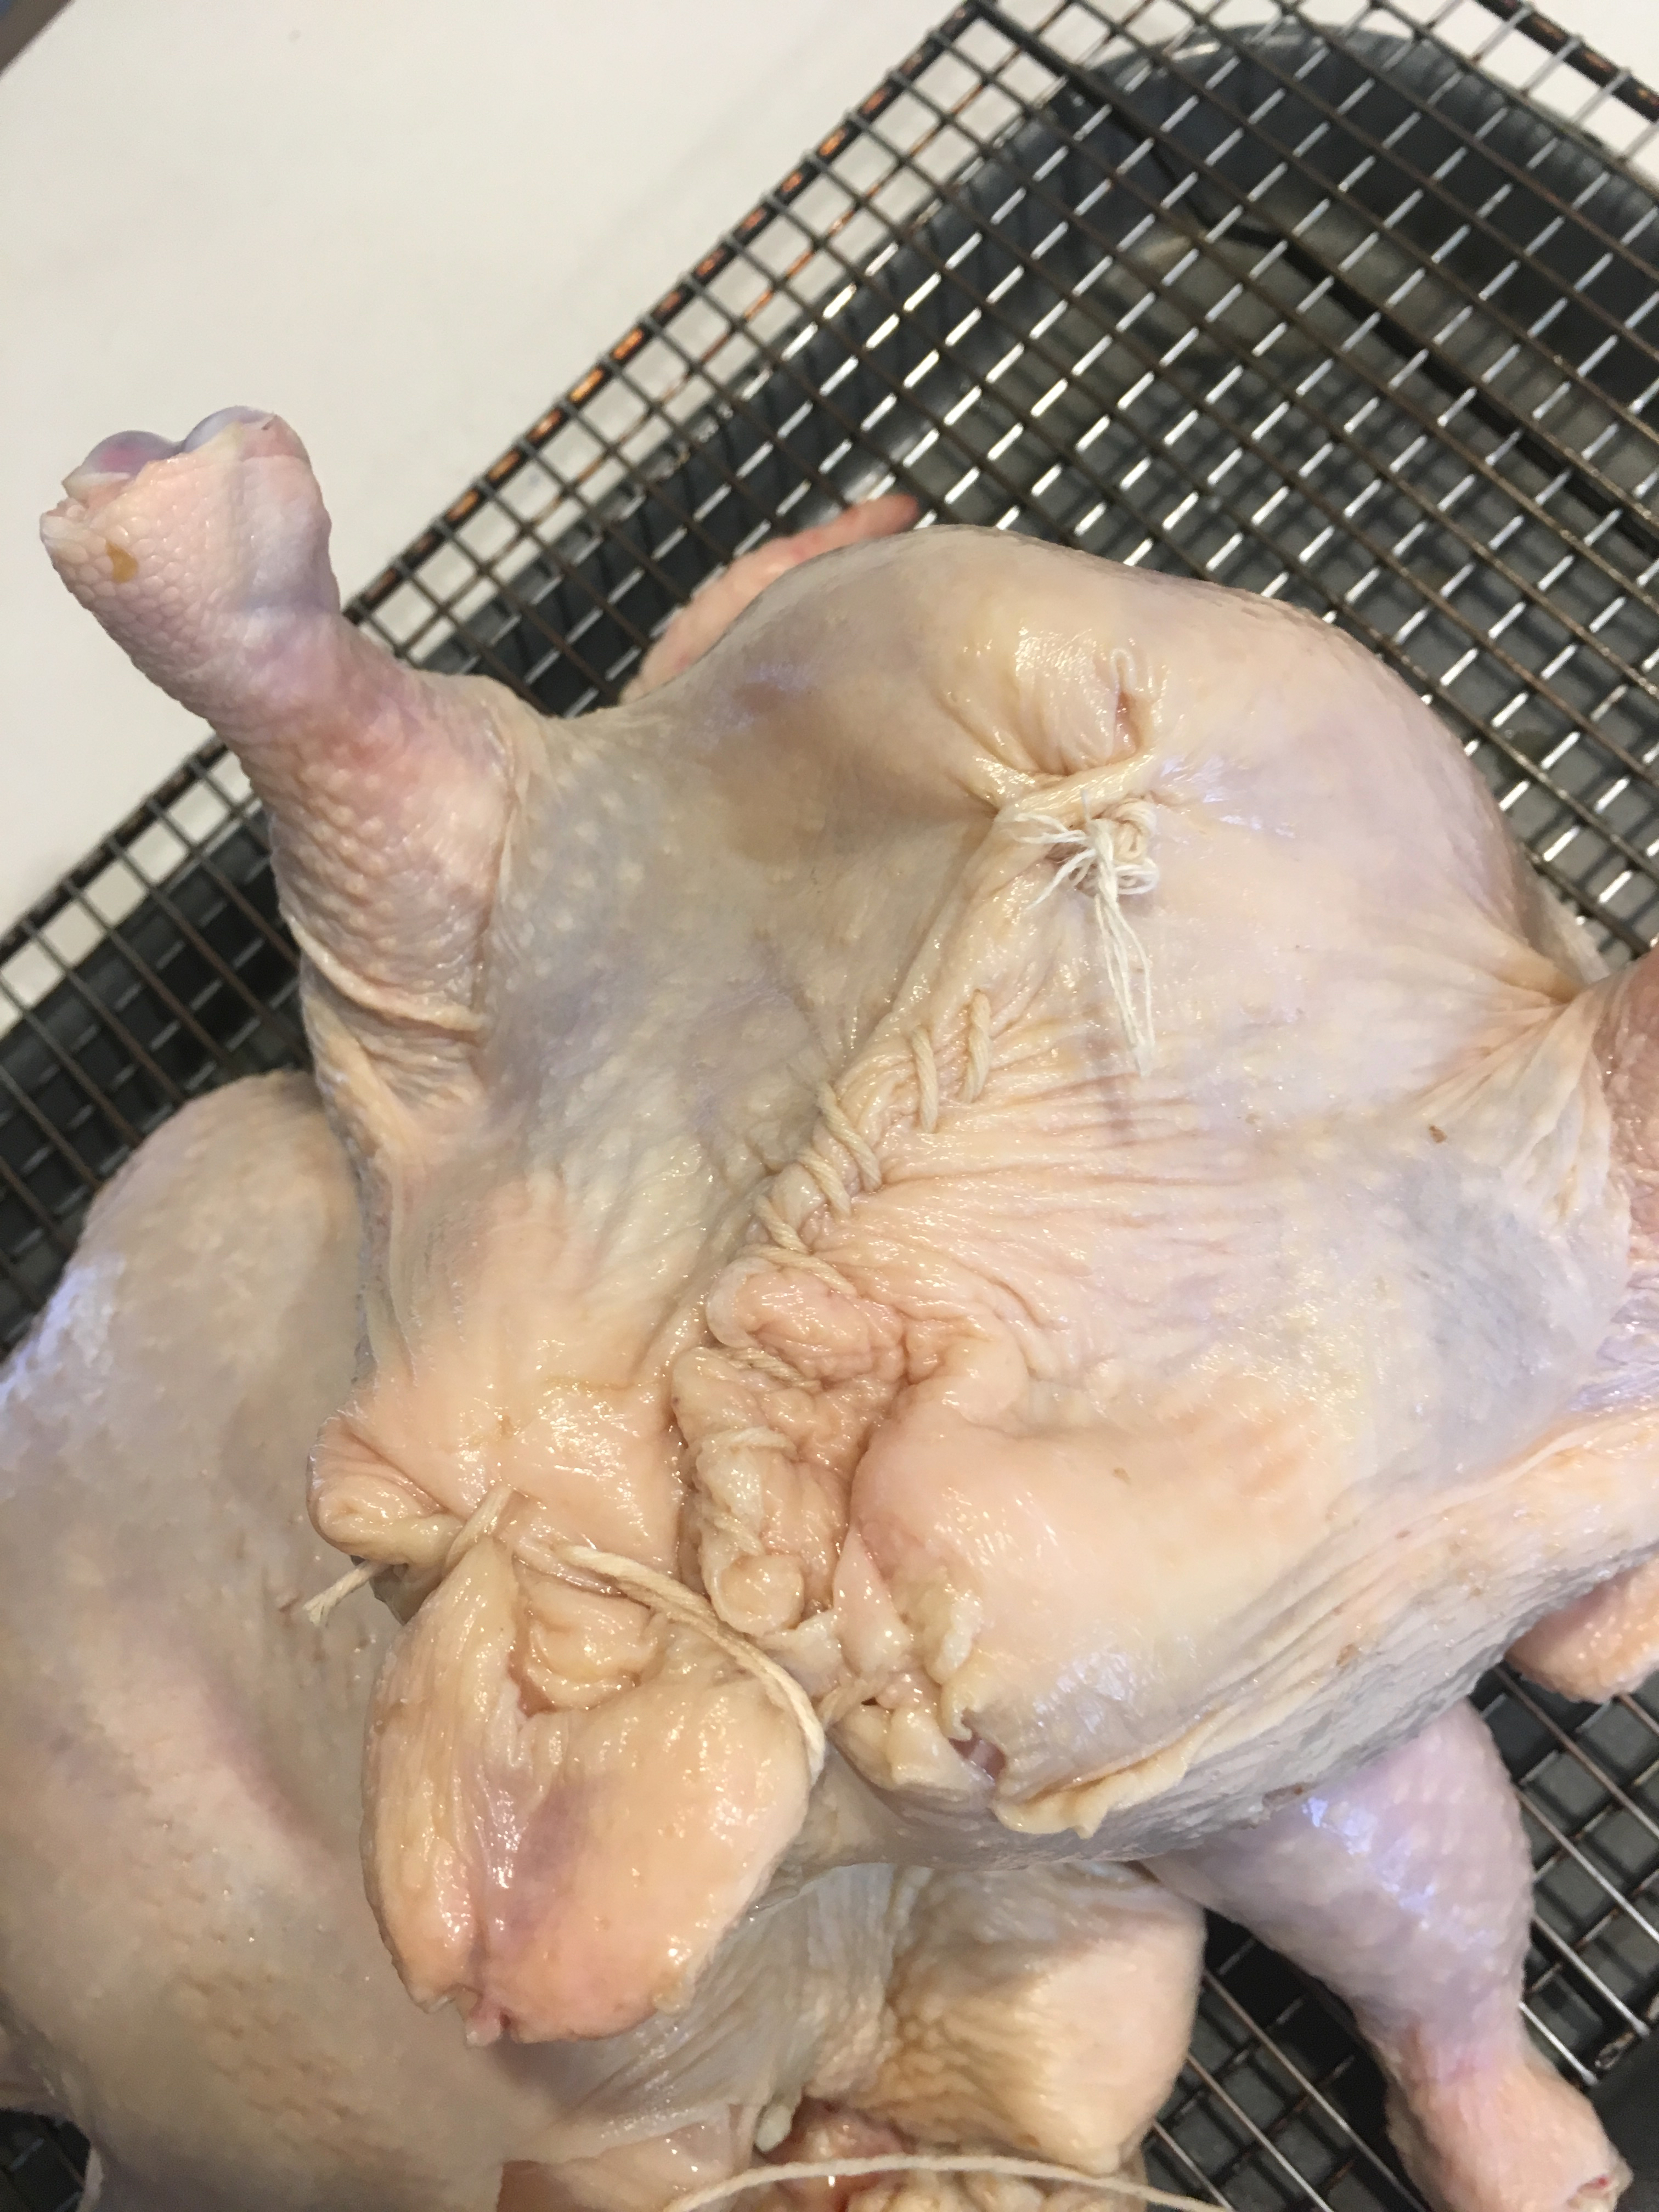
\includegraphics[width=0.25\textwidth]{\imageDir/\fileName/IMG_3217.jpg} &
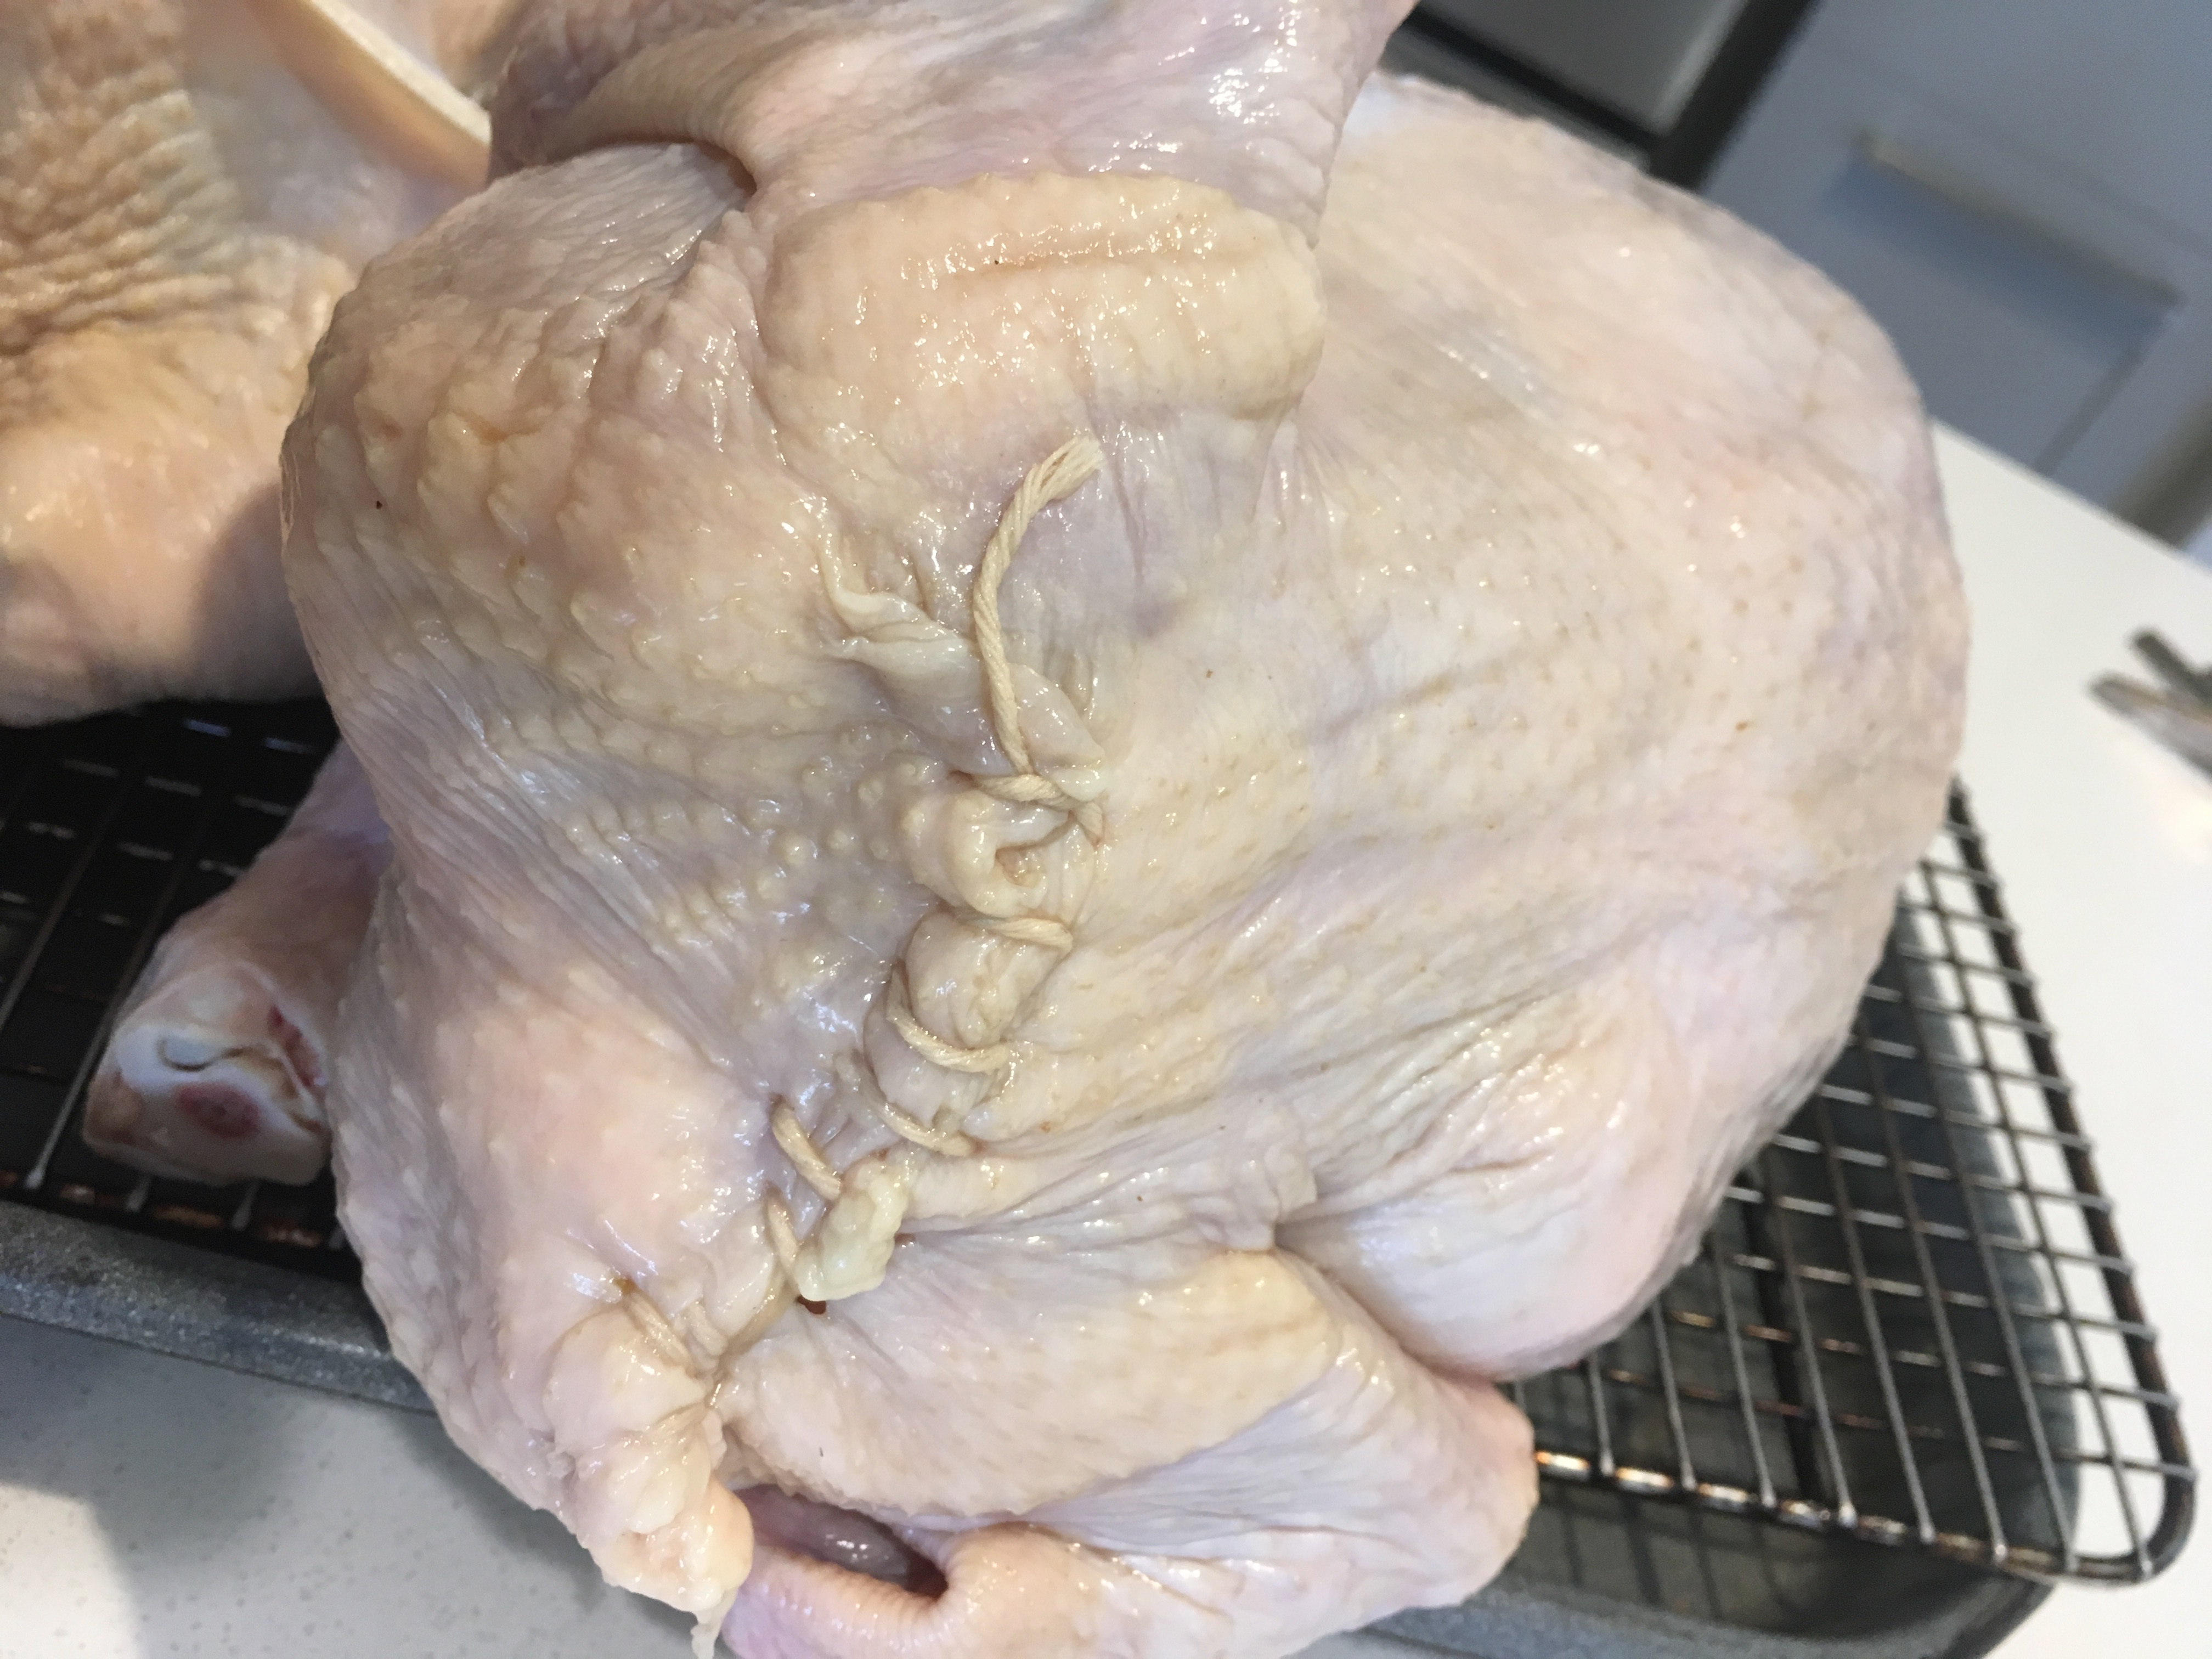
\includegraphics[width=0.25\textwidth]{\imageDir/\fileName/IMG_3218.jpg} &
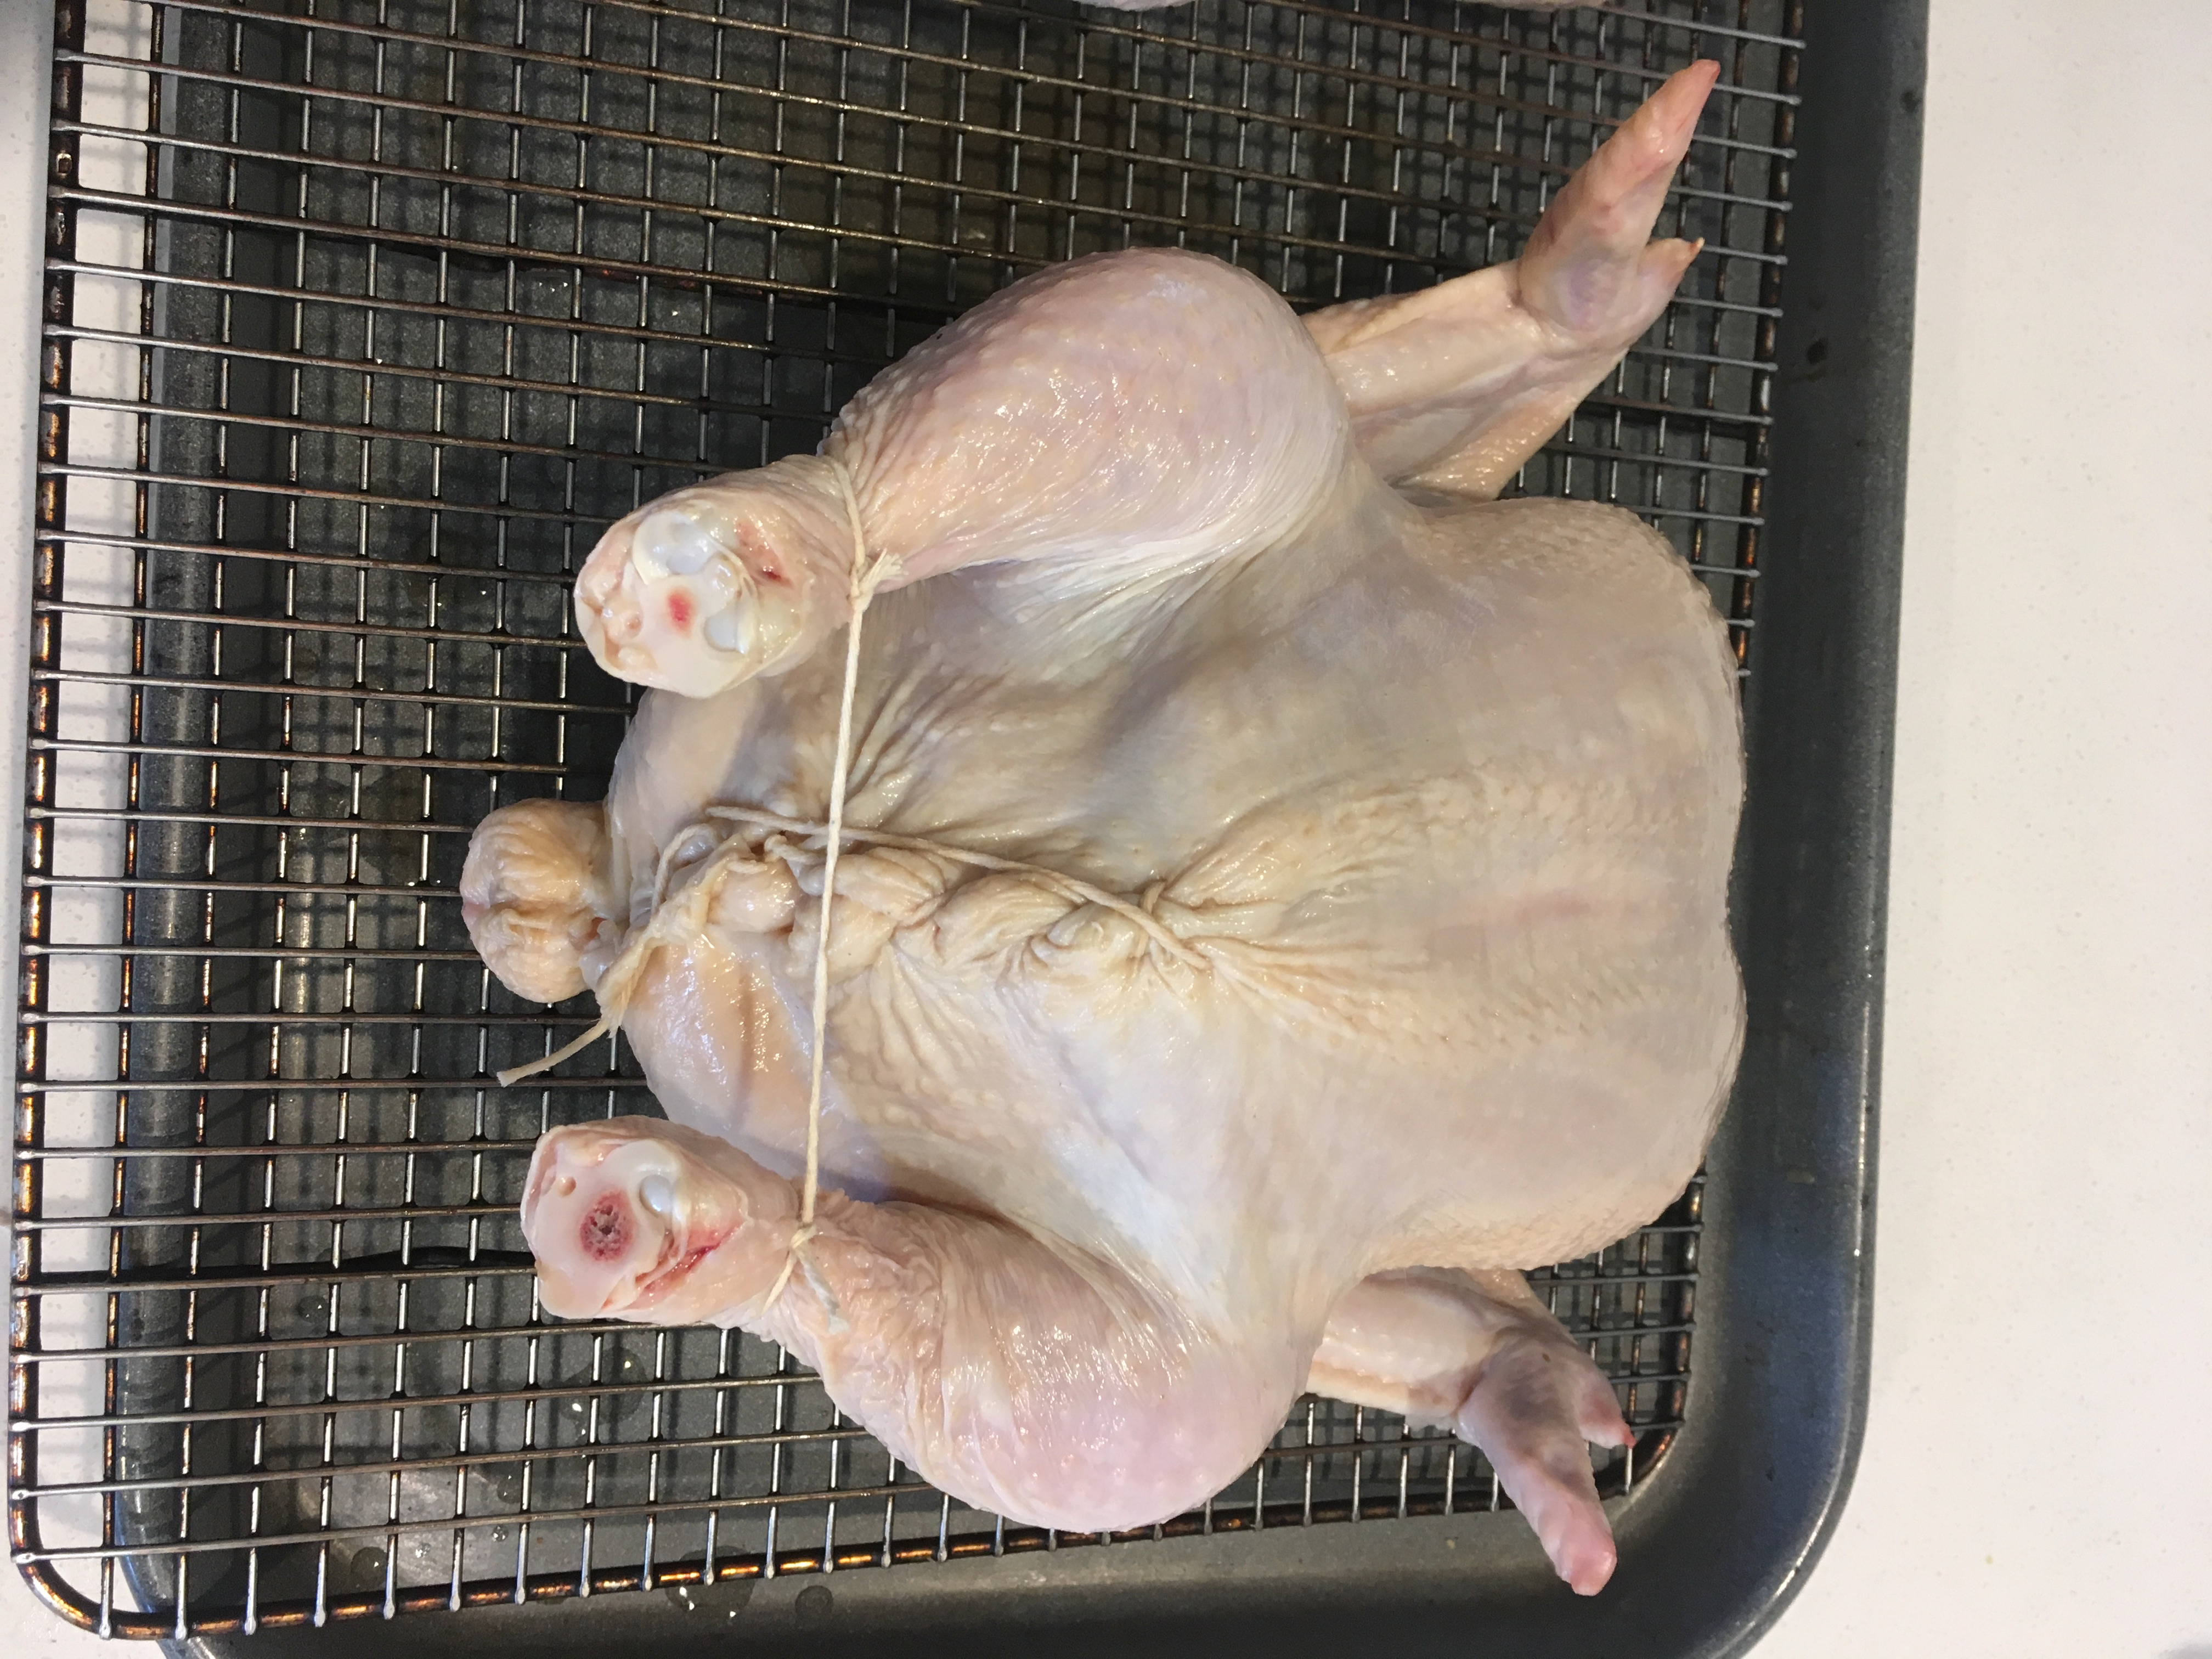
\includegraphics[width=0.25\textwidth]{\imageDir/\fileName/IMG_3219.jpg} \\
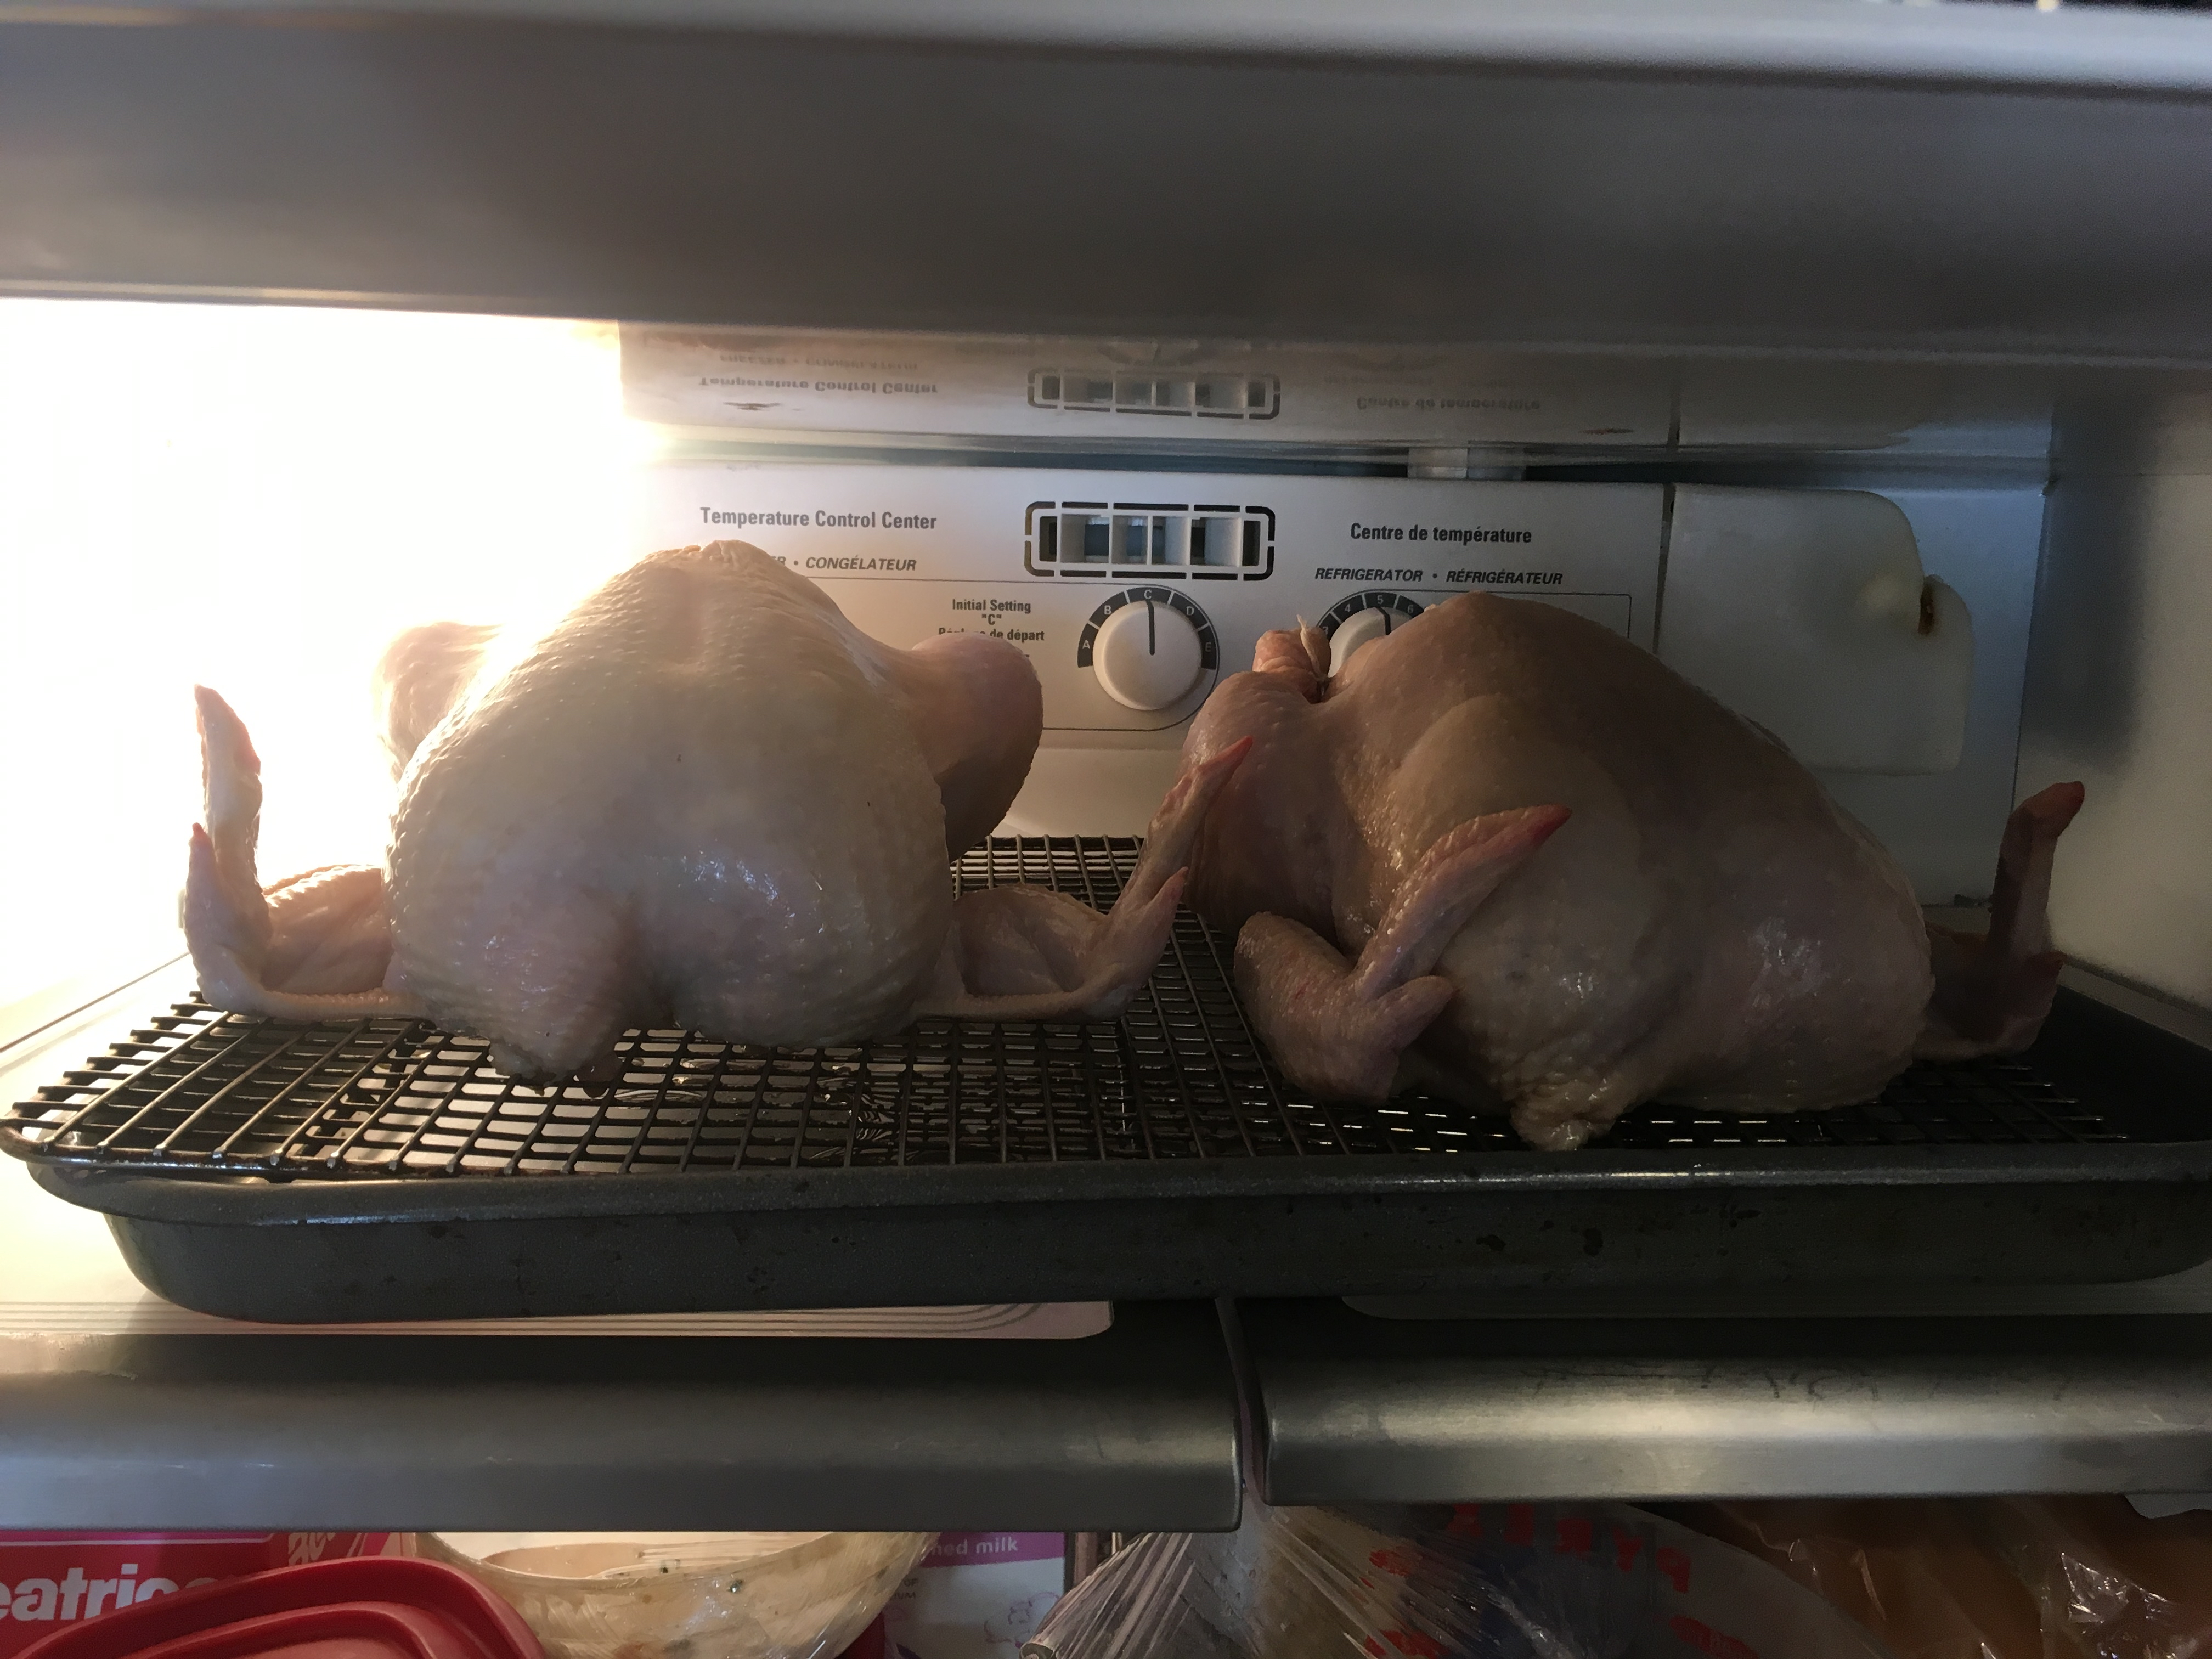
\includegraphics[width=0.25\textwidth]{\imageDir/\fileName/IMG_3220.jpg} &
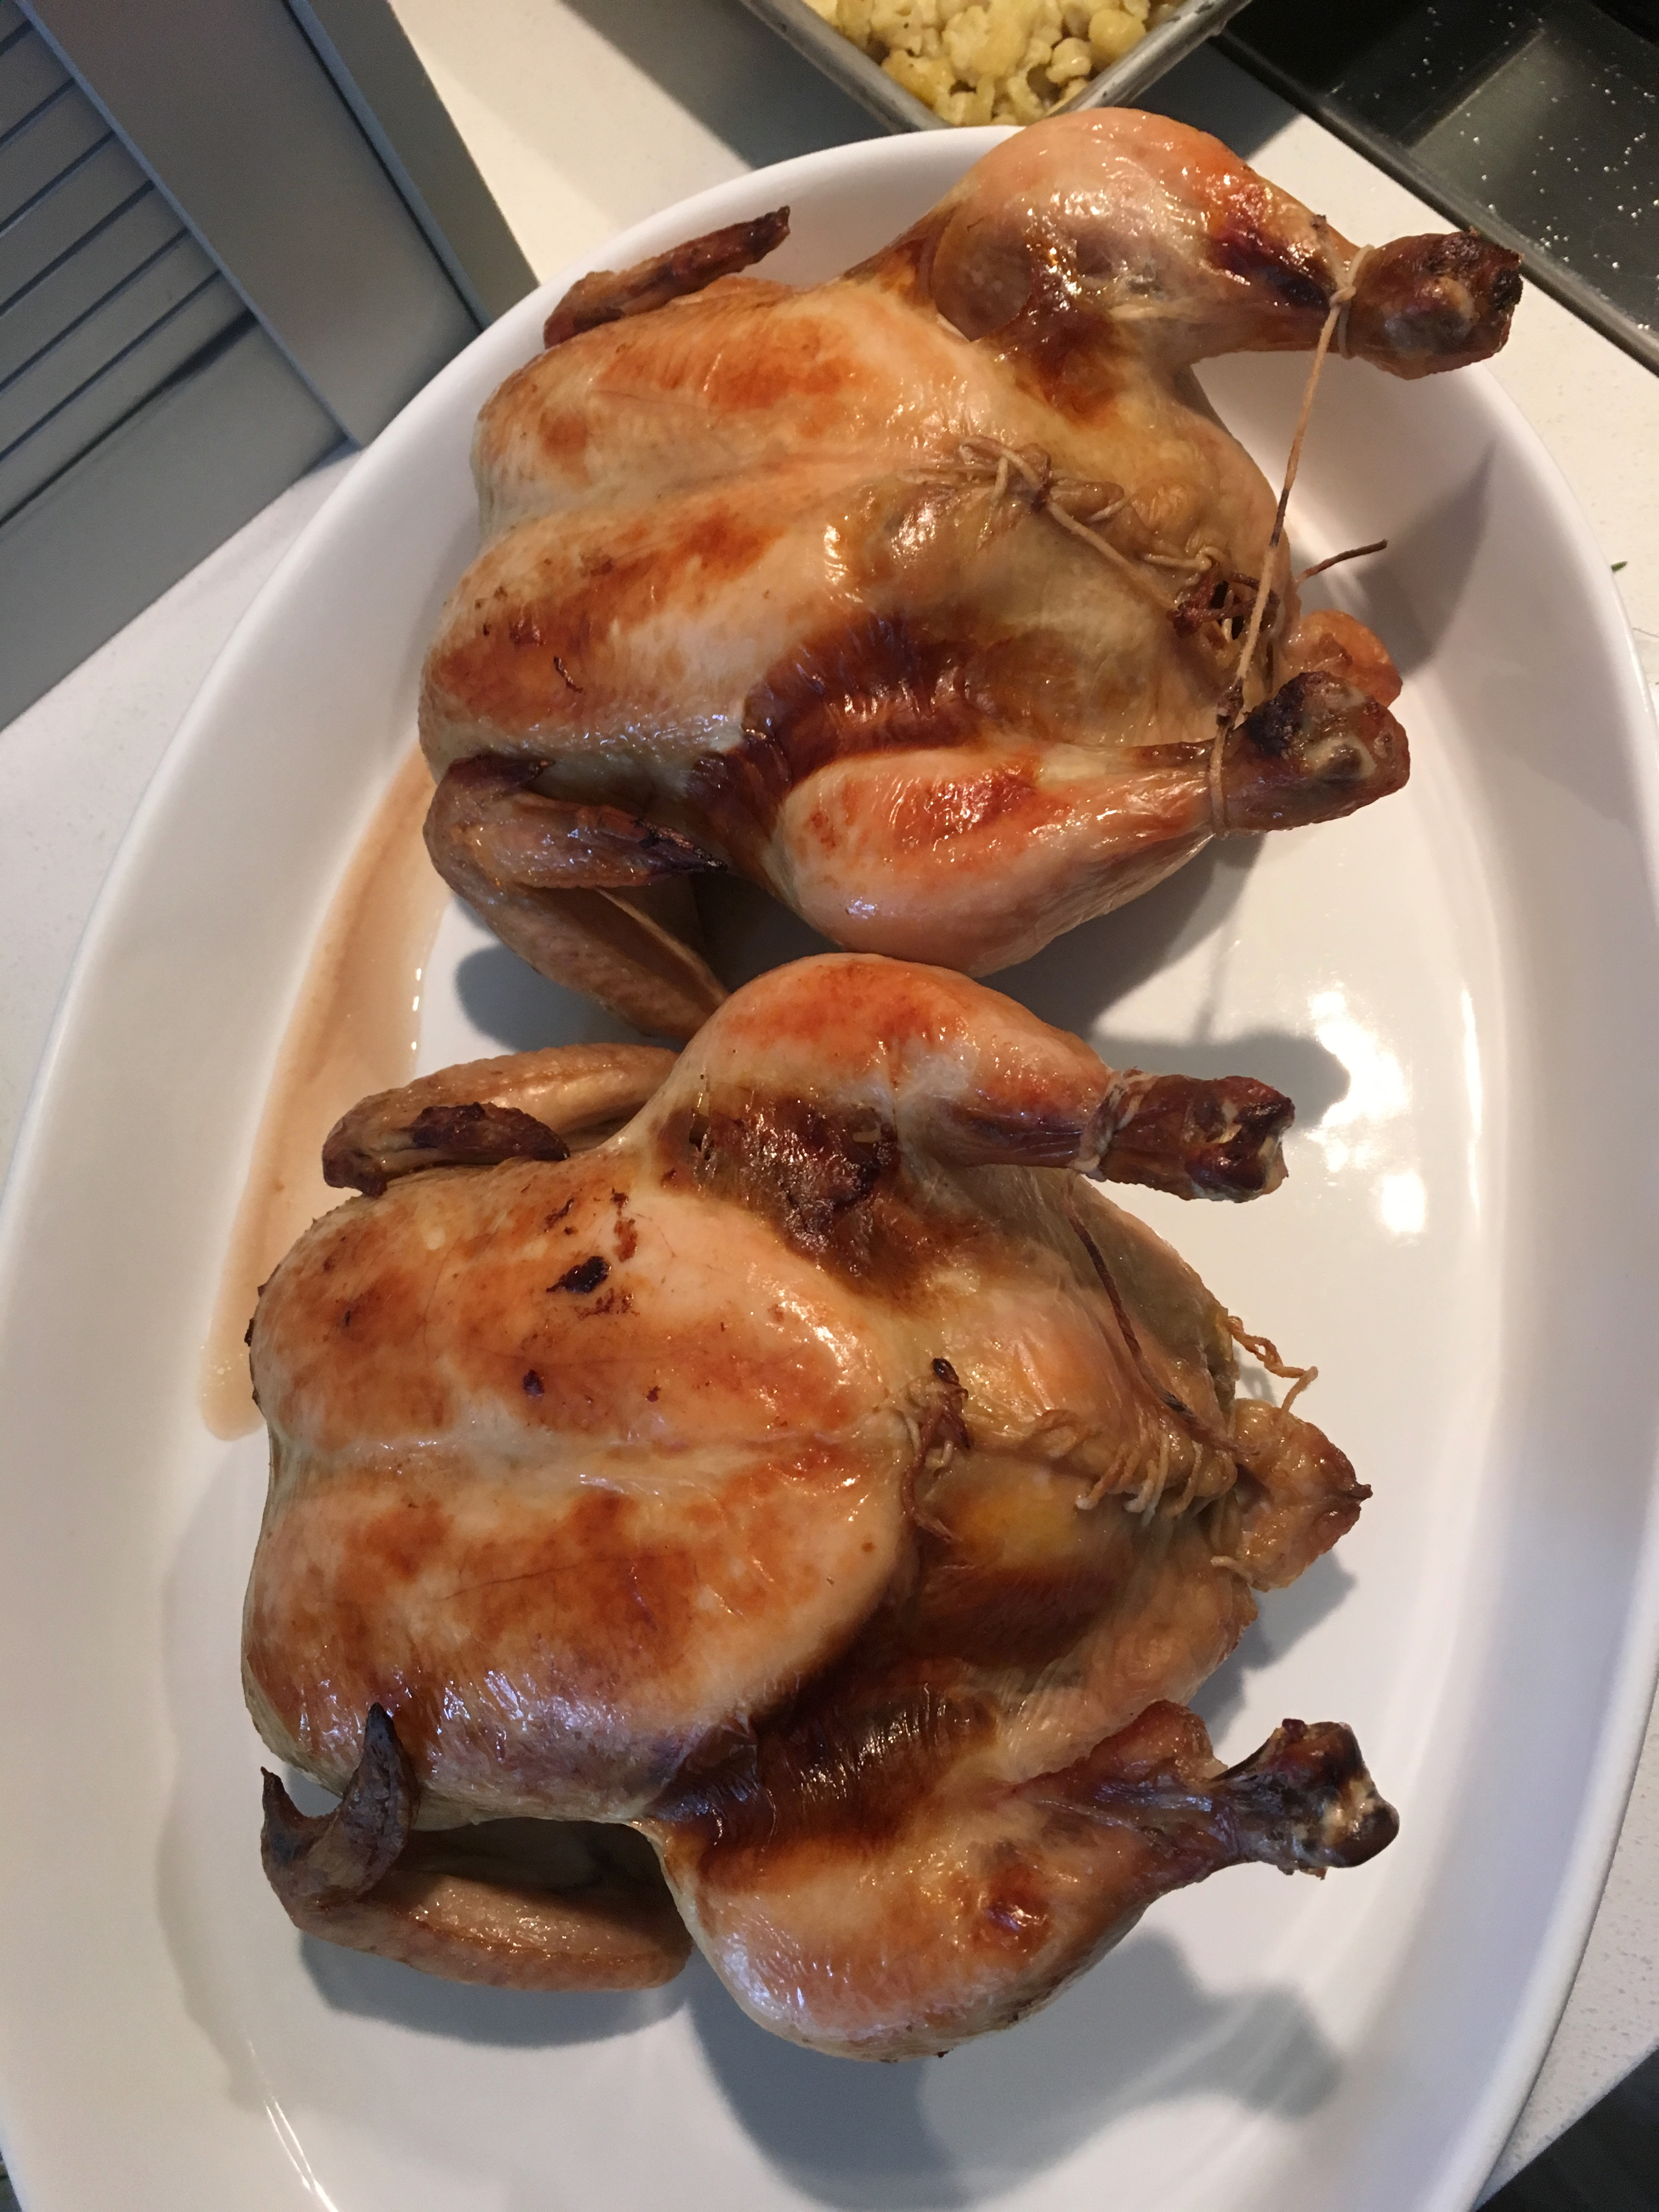
\includegraphics[width=0.25\textwidth]{\imageDir/\fileName/IMG_3228.jpg} \\
\end{tabular}
\end{table}


\end{document}
